\documentclass[a4paper,11pt]{article}

\usepackage{../../../Template/zemplate}

\usepackage{float}
\usepackage[dvipsnames]{xcolor}
\usepackage{hyperref}
%\setcounter{tocdepth}{2}
%\RequirePackage[acronym, toc]{glossaries}
\usepackage[acronym, toc]{glossaries}
%\newcommand{\glo}[1]{#1$_{\textit{G}}$}
% glossario
% per includerlo nel documento bisogna:
% 1. compilare una prima volta ManualeUtente.tex;
% 2. eseguire: 
% makeindex -s ManualeUtente.ist -t ManualeUtente.glg -o ManualeUtente.gls ManualeUtente.glo
% 3. eseguire:
%  makeindex -s ManualeUtente.ist -t ManualeUtente.alg -o ManualeUtente.acr ManualeUtente.acn
% 4. compilare due volte ManualeUtente.tex.
	
\docTitle{Manuale Utente}
\docVersion{2.0.0}
\docCreationDate{\frmdata{23}{03}{2017}}
\docLastUpdateDate{\frmdata{18}{08}{2017}}
\docStatus{Approvato}
\docEditors{Giulia Petenazzi}
\docVerificators{Jordan Gottardo}
\docApprovers{Marco Pasqualini}
\docUse{Esterno}
\docDestination{\Tullio \\ & \Cardin \\ & \zephyrus \\ & \riskapp}
\docJournal{
	2.0.0 & \frmdata{18}{08}{2017} & Marco Pasqualini & \responsabile & Approvazione del documento\\
	1.1.0 & \frmdata{18}{08}{2017} & Jordan Gottardo & \verificatore & Verifica del documento\\
	1.0.1 & \frmdata{16}{08}{2017} & Giulia Petenazzi & \programmatore & Aggiunte sezioni 9 e 10\\
	1.0.0 & \frmdata{06}{04}{2017} & Giovanni Prete & \responsabile & Approvazione del documento\\
	0.3.0 & \frmdata{05}{04}{2017} & Jordan Gottardo & \verificatore & Verifica del documento\\
	0.2.1 & \frmdata{04}{04}{2017} & Daniel De Gaspari & \progettista & Stesura glossario\\
	0.2.0 & \frmdata{01}{04}{2017} & Jordan Gottardo & \verificatore & Verifica del documento in
		forma parziale\\
	0.1.2 & \frmdata{28}{03}{2017} & Daniel De Gaspari & \progettista & Stesura sezione messaggi d'errore, segnalazione problemi e appendice validazioni\\
	0.1.1 & \frmdata{27}{03}{2017} & Daniel De Gaspari & \progettista & Stesura sezione gestione asset, nodo e arco\\
	0.1.0 & \frmdata{26}{03}{2017} & Jordan Gottardo & \verificatore & Verifica del documento in
	forma parziale\\
	0.0.3 & \frmdata{25}{03}{2017} & Giulia Petenazzi & \progettista & Stesura sezione interazione con la mappa\\
	0.0.2 & \frmdata{24}{03}{2017} & Giulia Petenazzi & \progettista & Stesura sezione introduzione, requisiti di sistema e azioni preliminari \\
	0.0.1 & \frmdata{23}{03}{2017} & Giulia Petenazzi & \progettista & Creazione template e indice\\
}
\newcommand\VRule[1][\arrayrulewidth]{\color{white} \vrule width 1pt}
\catcode`\_=12

\newglossaryentry{latex}
{
    name=latex,
    description={Is a mark up language specially suited for scientific documents}
}

\newglossaryentry{aaa}
{
	name=aaa,
	description={Is a mark up language specially suited for scientific documents}
}

\newglossaryentry{bbb}
{
	name=bbb,
	description={Is a mark up language specially suited for scientific documents}
}

\newglossaryentry{ccc}
{
	name=ccc,
	description={Is a mark up language specially suited for scientific documents}
}


\newglossaryentry{pippo}
{
	name=pippo,
	description={Is a mark up language specially suited for scientific documents}
}

\newglossaryentry{mario}
{
	name=mario,
	description={Is a mark up language specially suited for scientific documents}
}

\newglossaryentry{cappe}
{
	name=cappe,
	description={Is a mark up language specially suited for scientific documents}
}

\makeglossaries
\begin{document}
%\setcounter{secnumdepth}{2} % to block out subsubparagraph from showing out with its numbering (index etc.)

\newpage

\section{Introduzione}
	\subsection{Scopo del documento}
	Il presente documento rappresenta il Manuale Utente per il progetto \progetto{} sviluppato dal \mglo{Gruppo}{gruppo} \zephyrus{} per il proponente \riskapp.
	All'interno di esso vengono descritte le funzionalità offerte dal prodotto DeGeOP all'utente finale.
	
	\subsection{Scopo del prodotto}	\introScopo
	
	\subsection{Glossario}
	Allo scopo di rendere più semplice e chiara la comprensione del manuale, nel presente documento viene incluso un breve glossario.
	Per evidenziare un termine presente in tale documento, esso verrà marcato con il pedice \textsubscript{G}. Solo la prima occorrenza del termine in ogni sezione sarà marcata per non appesantire la lettura del documento.
	Tutti i termini del glossario evidenziati sono link ipertestuali al termine corrispettivo presente nel glossario.
\section{Requisiti di sistema}
Per poter utilizzare il prodotto DeGeOP è indispensabile una connessione internet.
	\subsection{Dispositivi e browser supportati}
		Al momento della stesura di questo documento l'applicazione è supportata dai seguenti dispositivi:
		\begin{itemize}
			\item \mglo{Windows}{Windows} v10;
			\item \mglo{Linux}{Linux} Ubuntu10.04 e Debian 8.0;
			\item \mglo{MacOS}{macOS} v10.2;
			\item Tablet - \mglo{Asus}{Asus} P01MA con sistema operativo Android 6.0.1;
			\item Tablet - \mglo{Ipad}{Ipad} Air 2 con sistema operativo \mglo{iOS}{iOS} 10.2.
		\end{itemize}
		e dai seguenti browser:
		\begin{itemize}
			\item \mglo{Chrome}{Chrome} v55;
			\item \mglo{Safari}{Safari} v10;
			\item \mglo{Firefox}{Firefox} v5.3;
			\item Firefox v50.
		\end{itemize}
	
		%\gls{latex}	
		%\gls{aaa}
	
\section{Azioni preliminari}
	%Descrizione delle azioni per entrare nell'applicazione quali:
	%sito dell'applicazione
	%login
	%pagine inerenti l'applicazione (praticamente tutti quello che esiste gia e che NON abbiamo fatto noi)
	%il cambio lingua va fatto qua??
	%	\gls{bbb}
DeGeOP è sviluppato su una single page che risulta essere parte integrante dell'attuale applicazione di \riskapp{}.
\\
Per accedere a DeGeOP, l'utente deve quindi effettuare una serie di operazioni:
\begin{itemize}
	\item aprire la \mglo{VirtualBox}{virtual box} fornita da \riskapp{};
	\item aprire il \mglo{Browser}{browser};
	\item effettuare l'accesso al sito di \riskapp{} cliccando sul segnalibro presente sulla barra dei segnalibri, utilizzando le seguenti credenziali:
	\begin{itemize}
		\item nome utente: admin;
		\item password: admin.
		\begin{figure}[H]
		\centering
		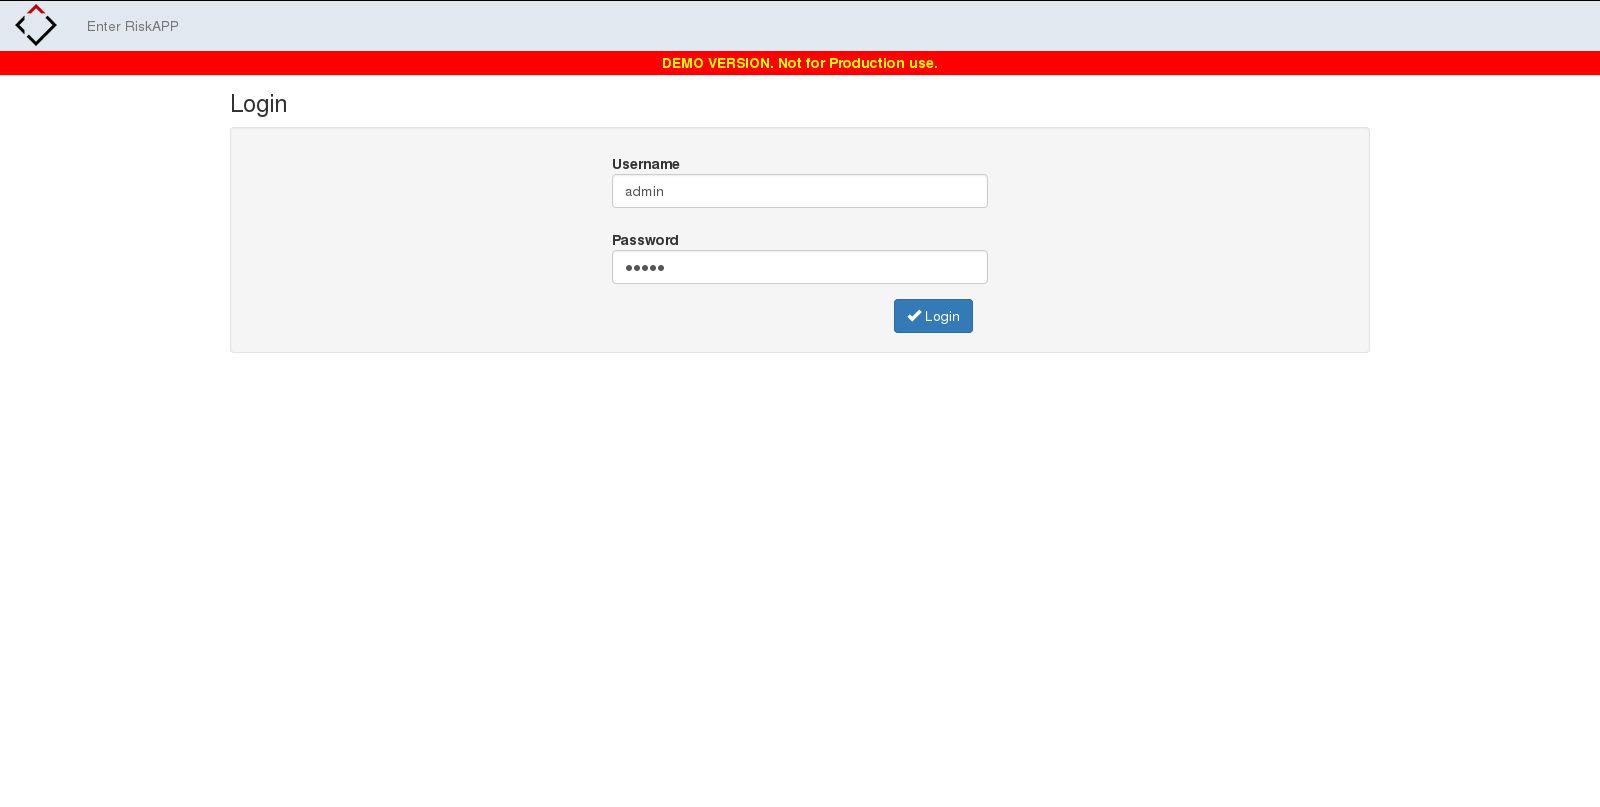
\includegraphics[width=\textwidth]{img/accessoDeGeOP/s1-login.png}
		\caption{Pagina di Login in RiskApp}
		\end{figure}
		
	\end{itemize}
	\item scegliere un cliente cliccando sul relativo pulsante "Edit";
		\begin{figure}[H]
		\centering
		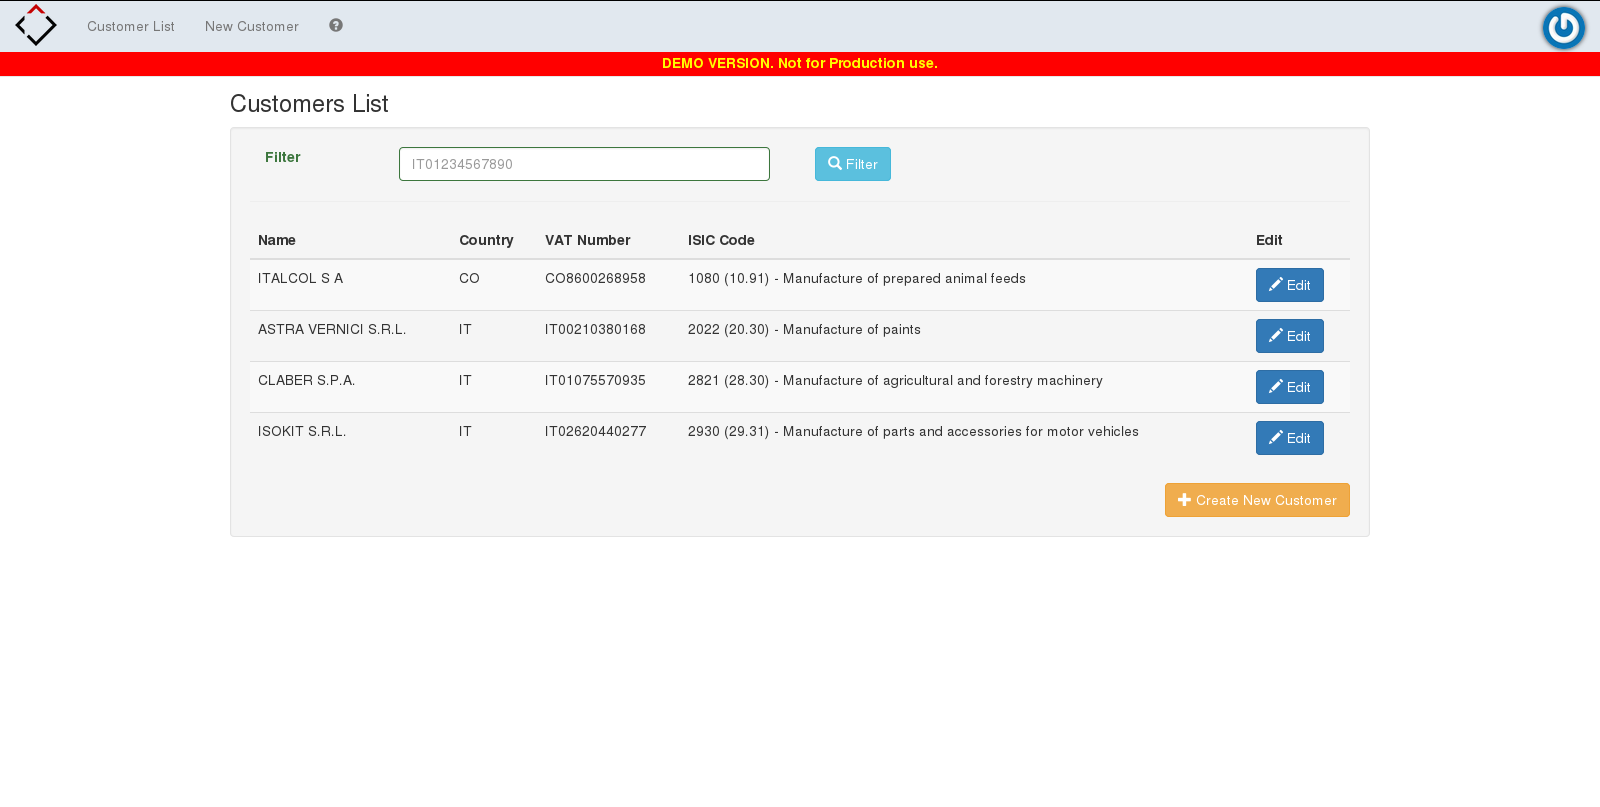
\includegraphics[width=\textwidth]{img/accessoDeGeOP/s2-select_customer.png}
		\caption{Scelta cliente in RiskApp}
		\end{figure}
	\item cliccare sulla scheda di menu denominata "Customer";
		\begin{figure}[H]
		\centering
		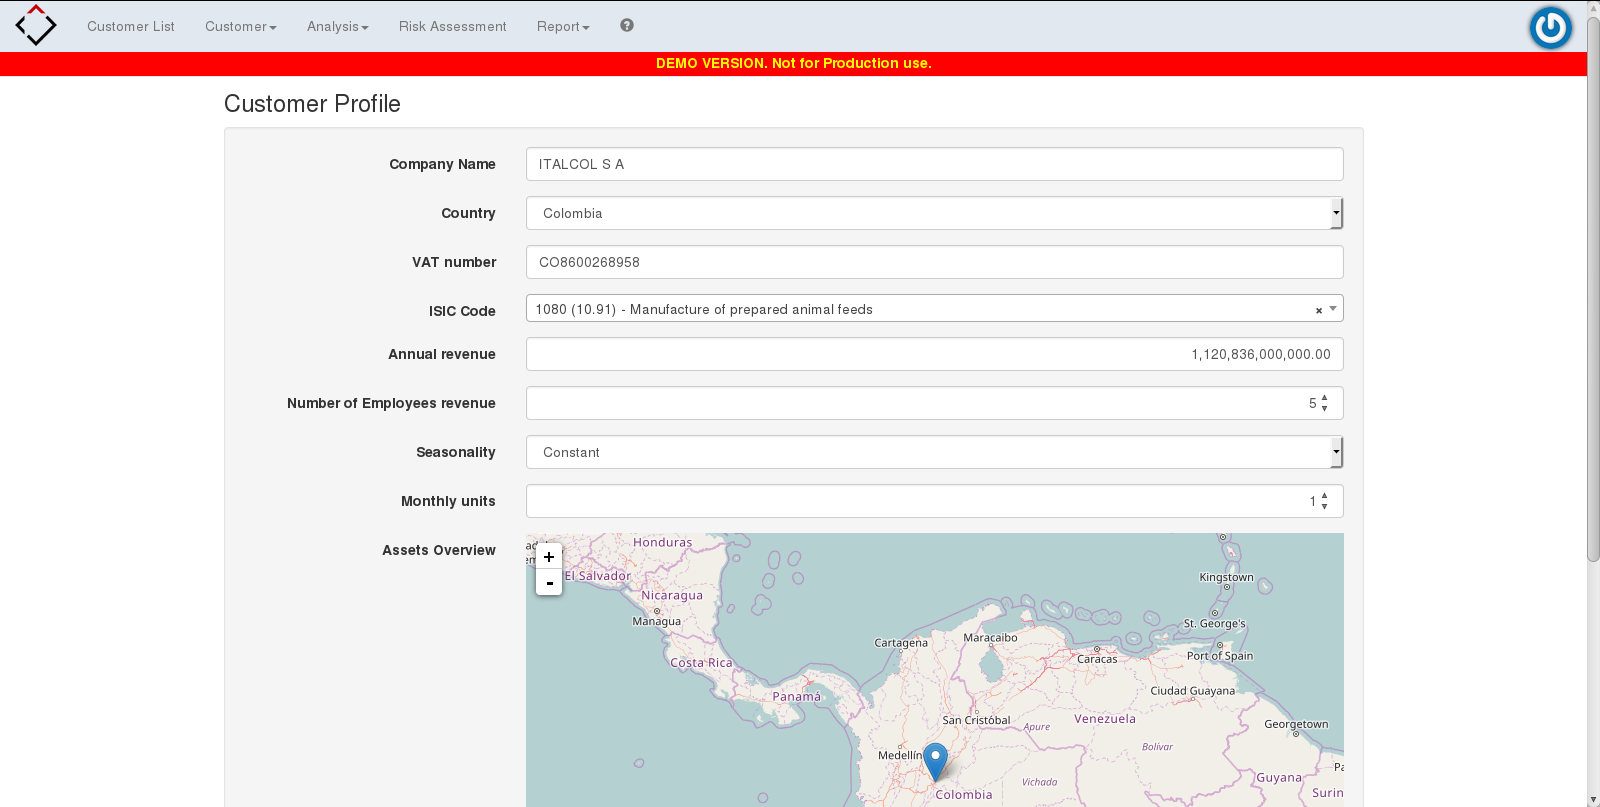
\includegraphics[width=\textwidth]{img/accessoDeGeOP/s3-customer_dashboard.png}
		\caption{Scheda di menu "Customer" in RiskApp}
		\end{figure}
	\item nel menu a tendina che compare, scegliere la voce "Processes";
		\begin{figure}[H]
		\centering
		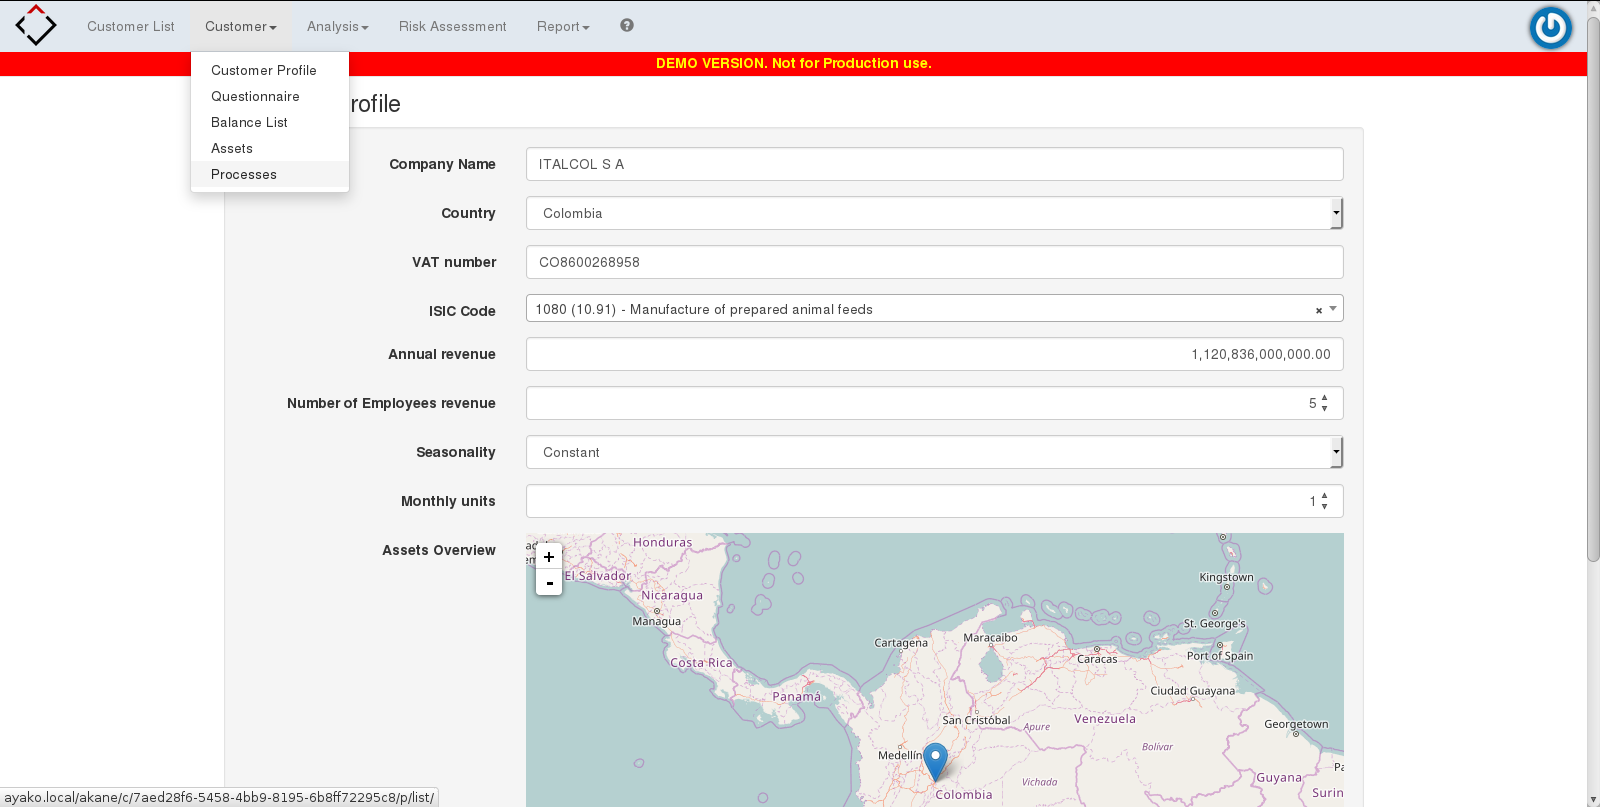
\includegraphics[width=\textwidth]{img/accessoDeGeOP/s4-select_menu_voice.png}
		\caption{Voce "Process" in RiskApp}
		\end{figure}
	\item scegliere un processo da modificare cliccando sul relativo pulsante "Edit";
		\begin{figure}[H]
		\centering
		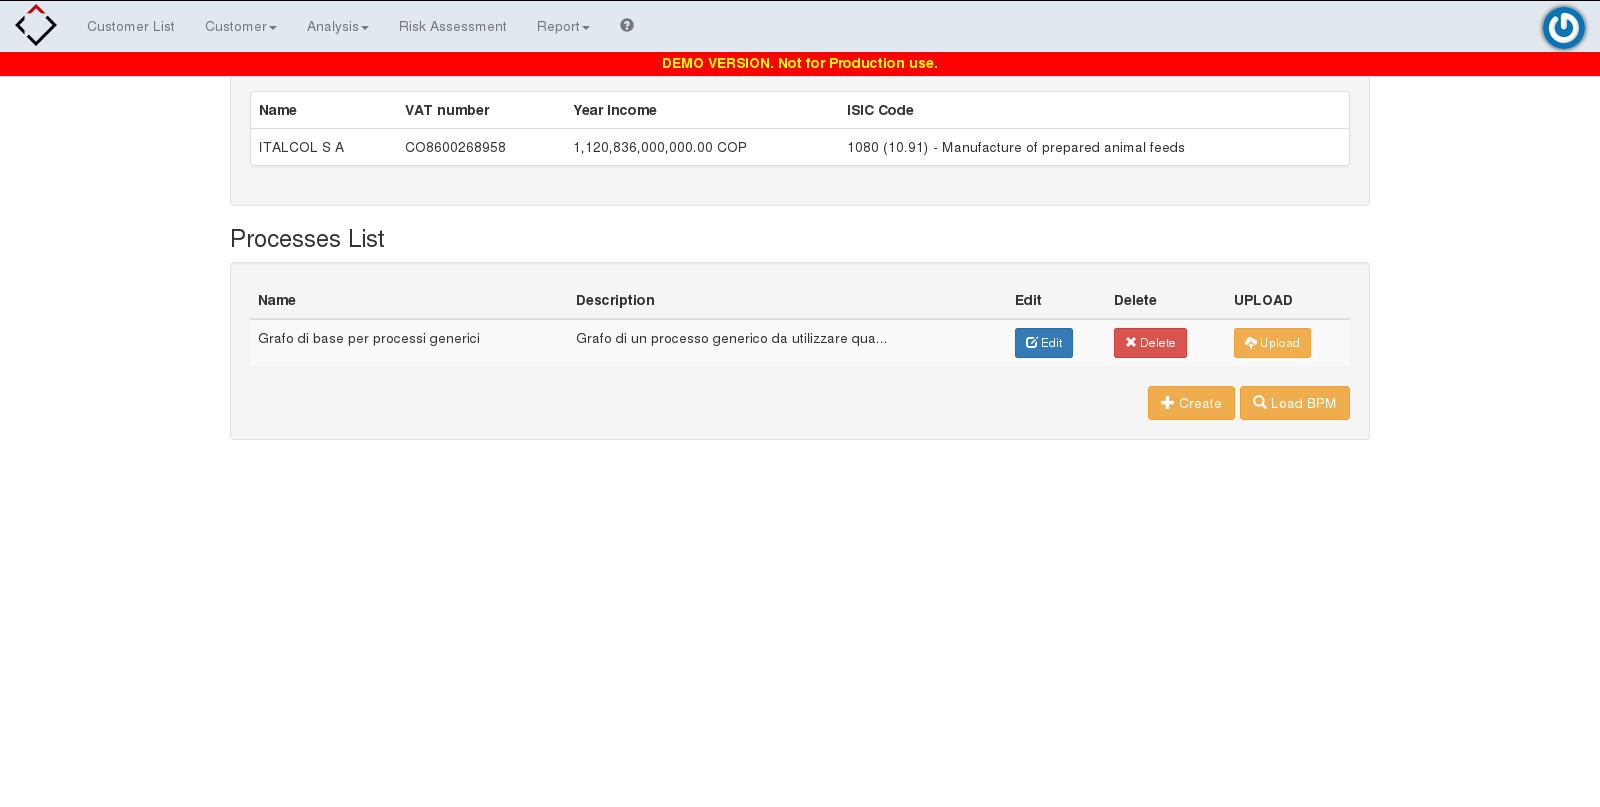
\includegraphics[width=\textwidth]{img/accessoDeGeOP/s5-select_process.png}
		\caption{Scelta processo in RiskApp}
		\end{figure}
	\item sei giunto alla single page DeGeOP.
		\begin{figure}[H]
		\centering
		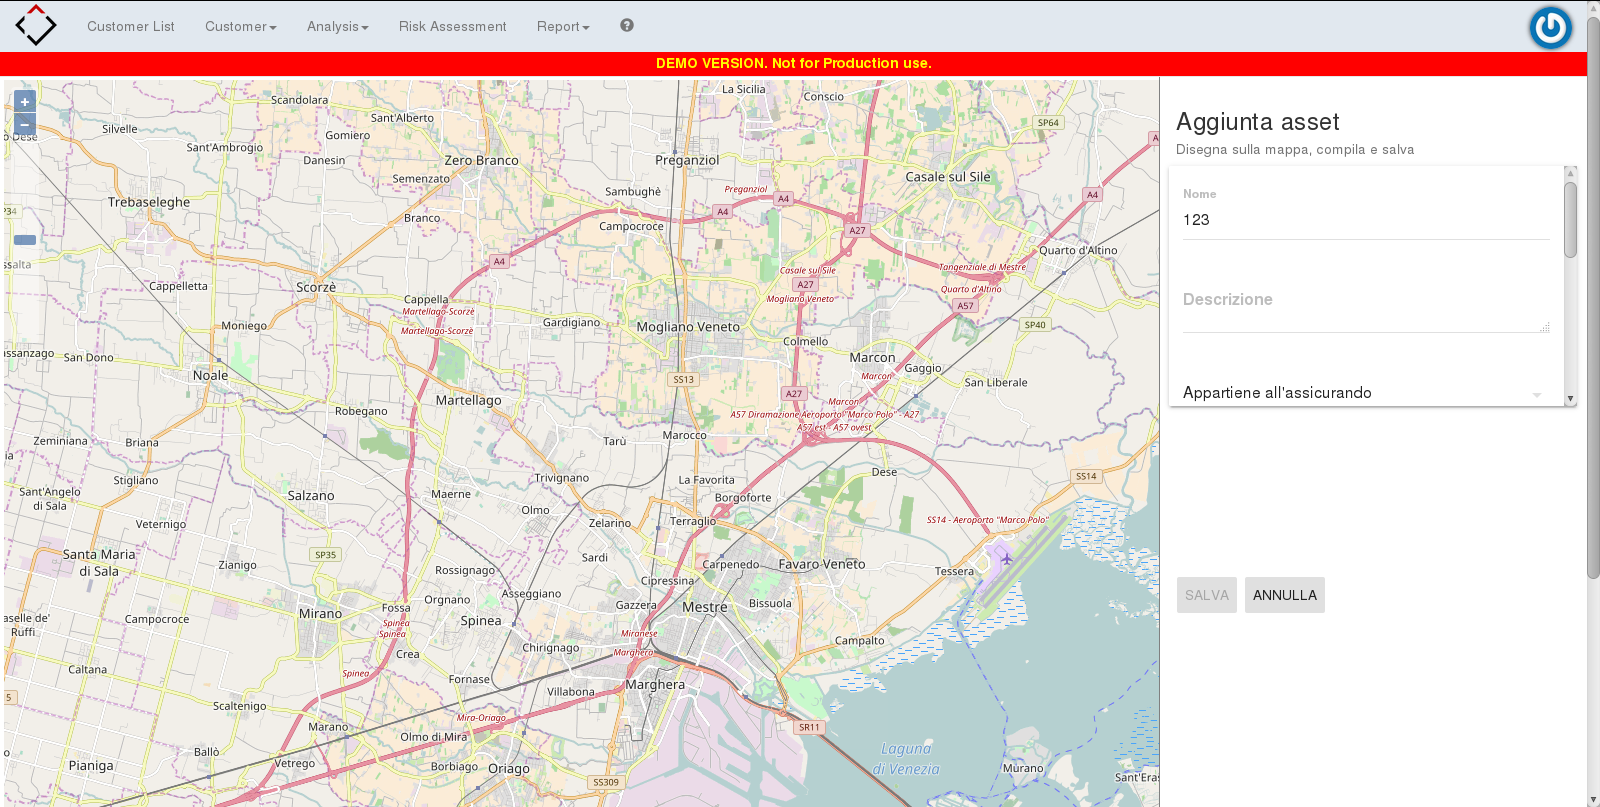
\includegraphics[width=\textwidth]{img/accessoDeGeOP/s6-DeGeOP.png}
		\caption{DeGeOP - visualizzazione di default}
		\end{figure}
\end{itemize}

\section{Introduzione App DeGeOP}
DeGeOP è sviluppato in una single-page che presenta un'interfaccia chiaramente divisa in due parti:
\begin{itemize}
	\item la mappa;
	\item la sidebar.
\end{itemize}
L'utente potrà:
\begin{itemize}
	\item interagire con la mappa:
	\begin{itemize}
		\item aumentando/diminuendo il livello di zoom;
		\item spostandosi sulla mappa.
	\end{itemize}
	\item aggiungere \mglo{Asset}{asset}, \mglo{Nodi}{nodi}, \mglo{Archi}{archi};
	\item visualizzare i dettagli di asset, nodi, archi;
	\item modificare asset, nodi, archi;
	\item eliminare asset, nodi, archi.
\end{itemize}
\section{Interazione con la mappa}
Per quanto riguarda l'interazione con la mappa è possibile:
\begin{itemize}
	\item aumentare /diminuire il livello di zoom;
	\item spostarsi sulla mappa.
\end{itemize}

\subsection{Aumentare/diminuire il livello di zoom)}
Per modificare il livello di zoom è possibile:
\begin{itemize}
	\item cliccare sui pulsanti "+" e "-" in alto a sinistra della mappa;
	\item muovere il segnaposto sullo slider;
	\item utilizzare la gesture "pinch" (solo in caso di fruizione da tablet).
\end{itemize}

\begin{figure}[H]
\centering
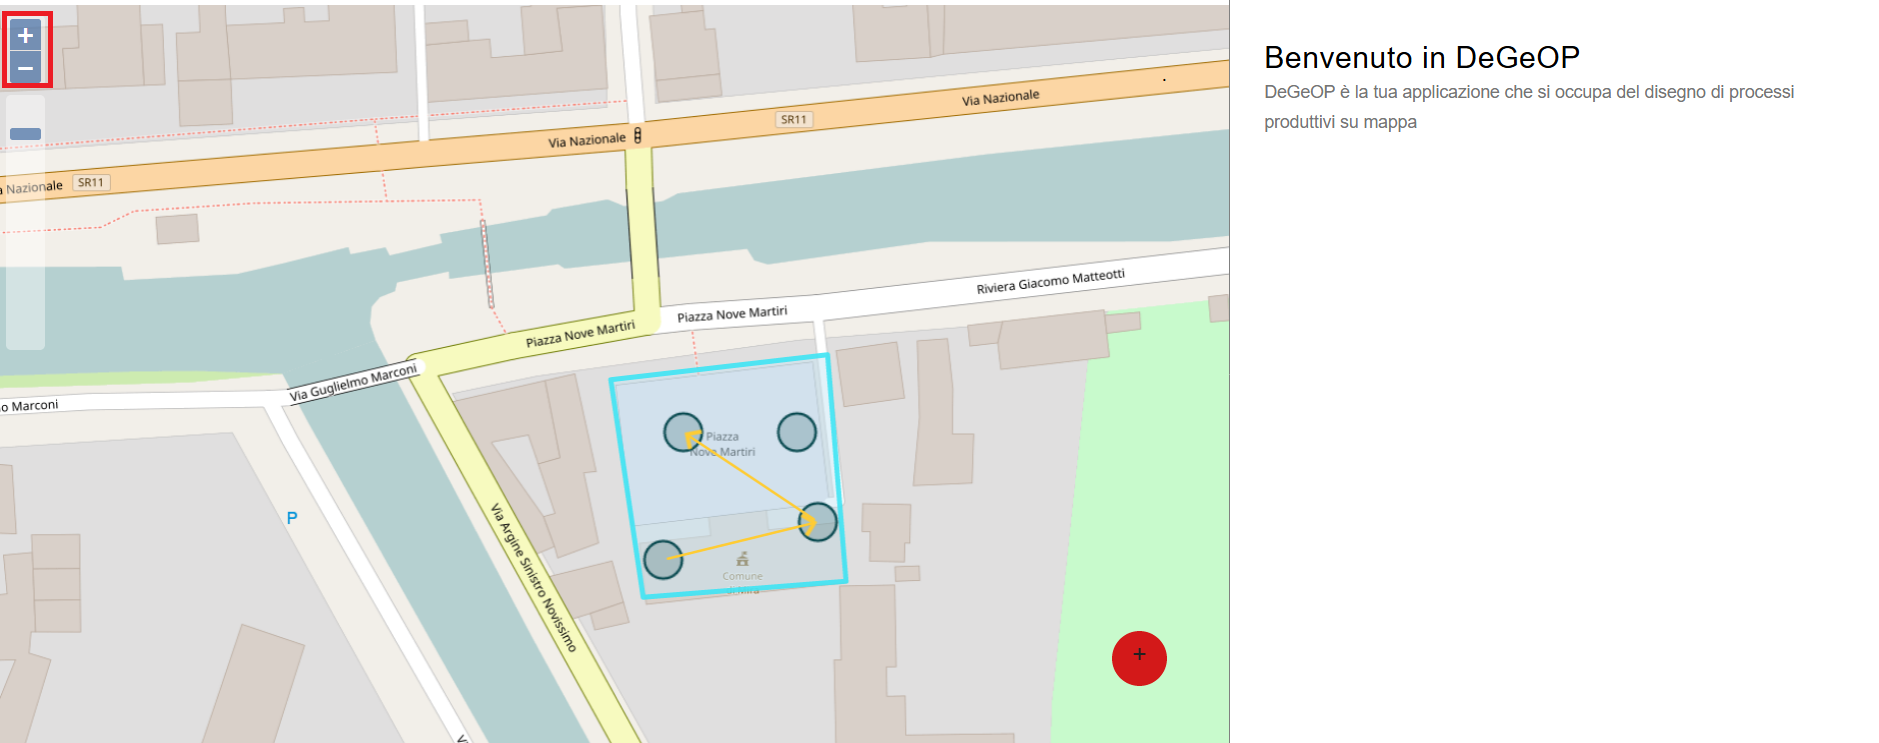
\includegraphics[width=\textwidth]{img/zoom.png}
\caption{Zoom}
\end{figure}

\subsection{Spostarsi sulla mappa}
Per spostarsi sulla mappa è possibile:
\begin{itemize}
	\item spostandosi sulla mappa trascinandola;
	\item utilizzare la \mglo{Gesture}{gesture} "drag" (solo in caso di fruizione da tablet).
\end{itemize}
\section{Gestione asset}
	Per quanto riguarda la gestione degli \mglo{Asset}{asset} l'utente ha la possibilità di:
	\begin{itemize}
		\item aggiungere un asset;
		\item visualizzare i dettagli relativi a un certo asset presente;
		\item modificare un asset presente;
		\item eliminare un asset presente.
	\end{itemize}

\subsection{Aggiunta di un asset}
	Per aggiungere un asset si deve:
	\begin{itemize}
		\item cliccare sul pulsante "+" in basso a destra della mappa;
		\item selezionare la voce "Aggiungi asset";
		\item disegnare il perimetro dell'asset sulla mappa. E' possibile apporre gli spigoli del perimetro cliccando direttamente sulla mappa. Il perimetro dell'asset deve essere correttamente chiuso, facendo coincidere l'ultimo spigolo del perimetro col primo;
		\item compilare i campi (tutti) rispettando i vincoli esposti nell'apposita appendice \nameref{Validazioni};
		\item cliccare sul pulsante "Salva", che verrà abilitato solo nel momento in cui tutte le operazioni sopra descritte sono state eseguite in maniera corretta.
	\end{itemize}
	
	\begin{figure}[H]
	\centering
	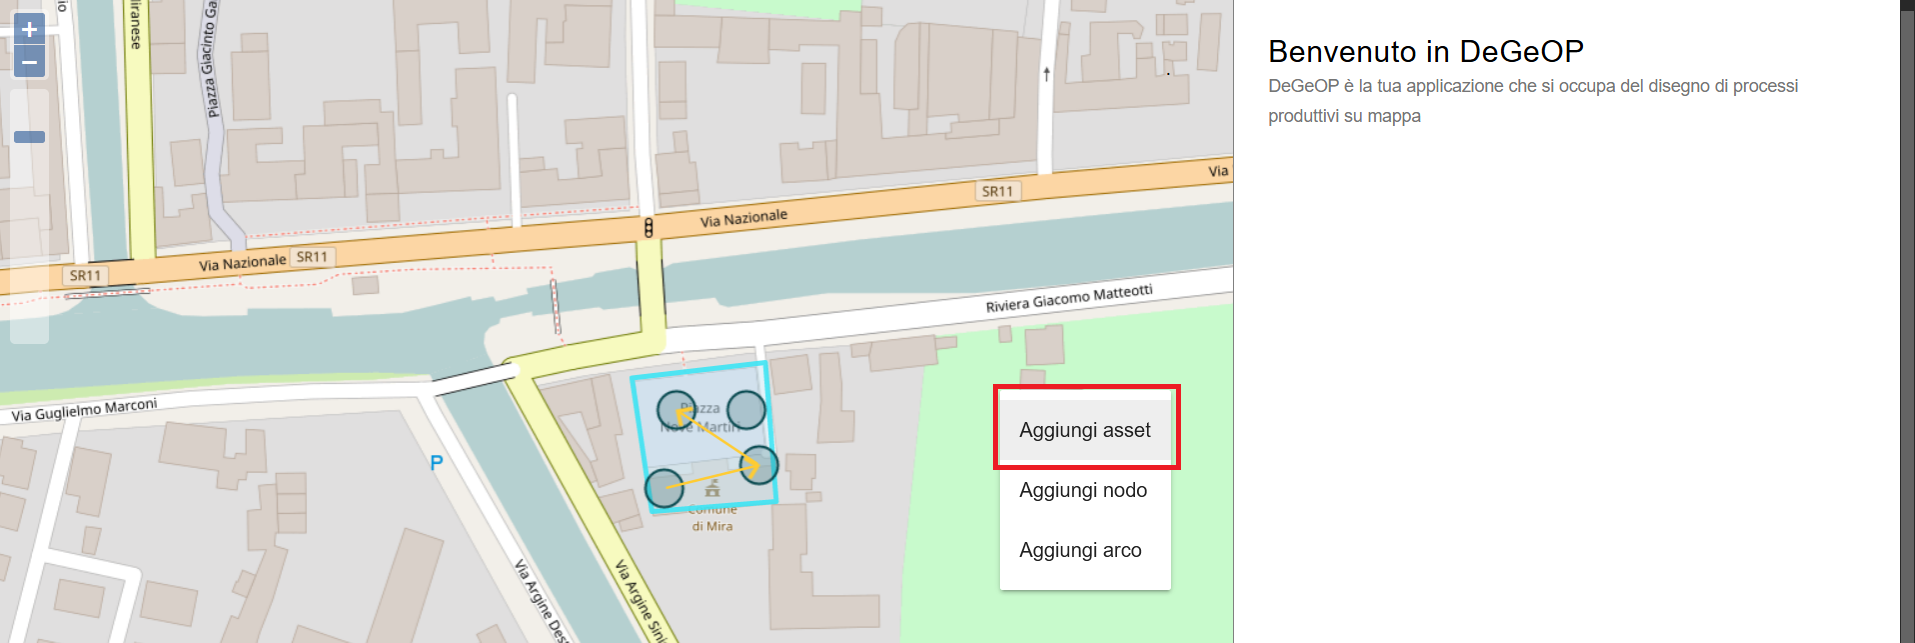
\includegraphics[width=\textwidth]{img/menu_aperto_asset_hover.png}
	\caption{Menu di aggiunta}
	\end{figure}
	
	\begin{figure}[H]
	\centering
	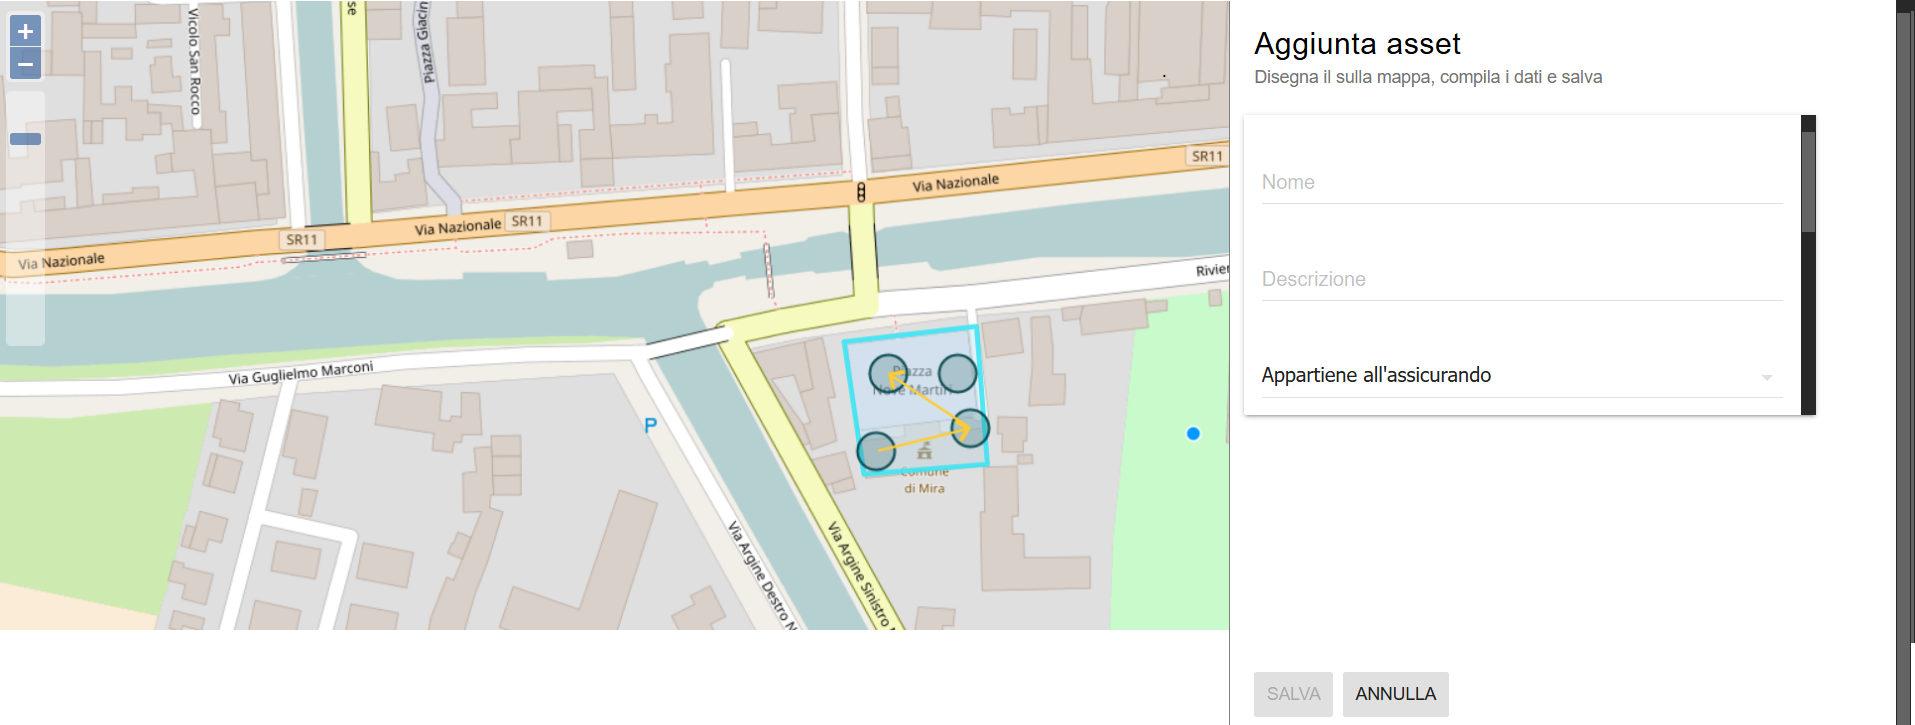
\includegraphics[width=\textwidth]{img/aggiunta_asset.png}
	\caption{Aggiunta di un asset}
	\end{figure}

\subsection{Visualizzazione dei dettagli di un asset}
	Per visualizzare i dettagli di un asset si deve:
	\begin{itemize}
		\item selezionare l'asset che si intende modificare cliccando direttamente su quell'asset dalla mappa.
	\end{itemize}
	
	\begin{figure}[H]
	\centering
	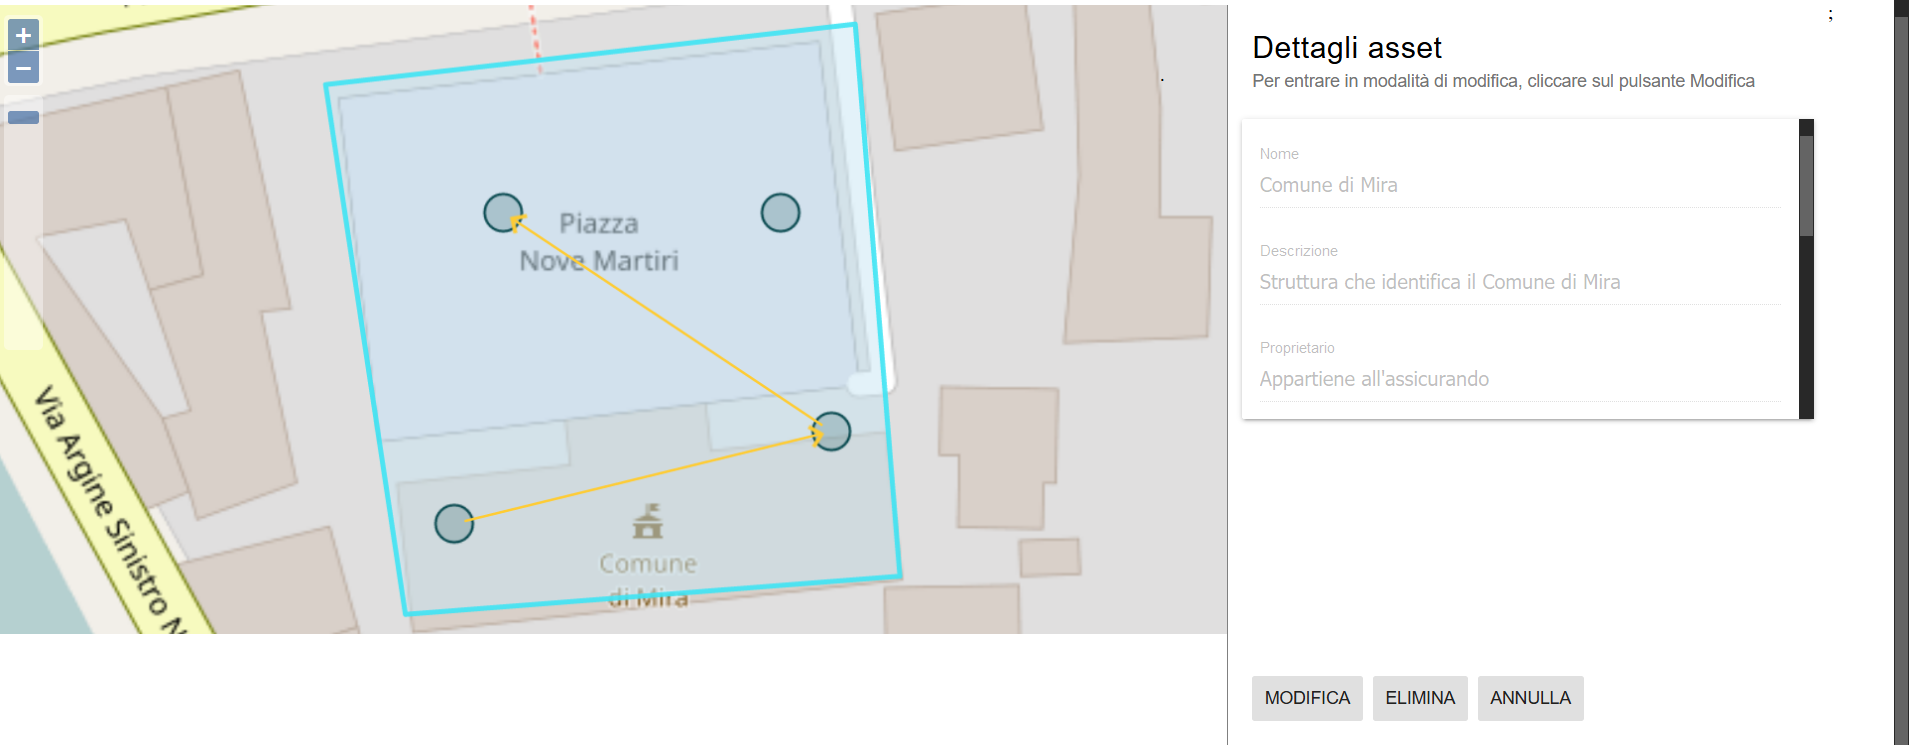
\includegraphics[width=\textwidth]{img/visualizzazione_asset.png}
	\caption{Visualizzazione dettagli di un asset}
	\end{figure}

\subsection{Modifica di un asset}
	Per modificare un asset si deve:
	\begin{itemize}
		\item selezionare l'asset che si intende modificare cliccando direttamente sulla mappa;
		\item cliccare sul pulsante "Modifica" in basso sulla sidebar;
		\item eventualmente ridisegnare il perimetro dell'asset sulla mappa. E' possibile apporre gli spigoli del perimetro cliccando direttamente sulla mappa. Il nuovo perimetro andrà in automatico a sovrascrivere quello precentemente presente. Il perimetro dell'asset deve essere correttamente chiuso, facendo coincidere l'ultimo spigolo del perimetro col primo;
		\item eventualmente modificare i campi rispettando i vincoli esposti nell'apposita appendice \nameref{Validazioni};
		\item cliccare sul pulsante "Salva", che verrà abilitato solo nel momento in cui tutte le operazioni sopra descritte sono state eseguite in maniera corretta.
	\end{itemize}
	
	\begin{figure}[H]
	\centering
	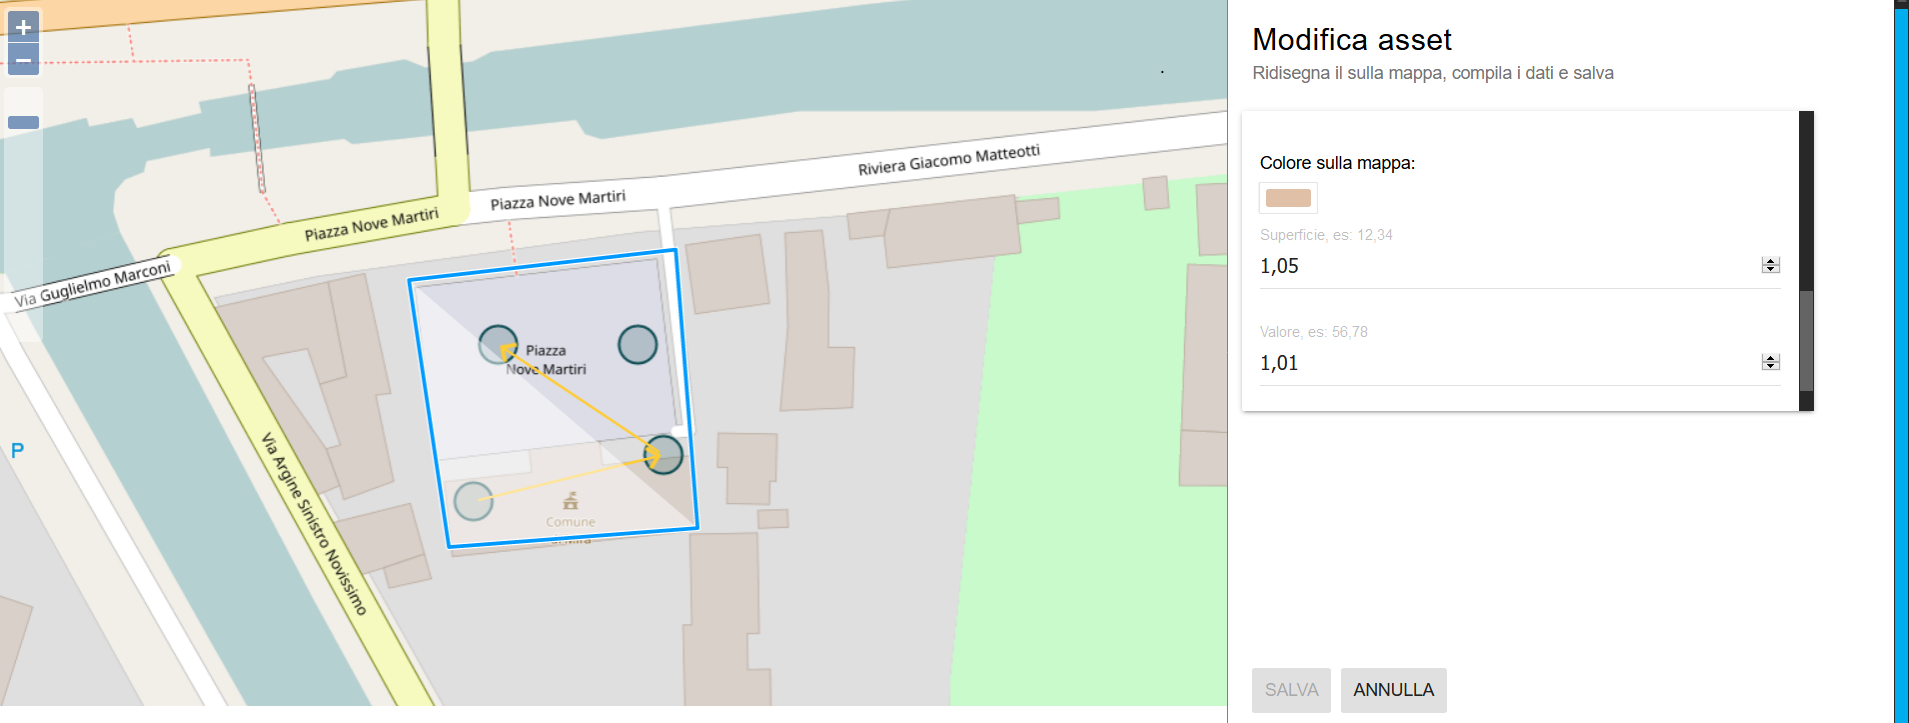
\includegraphics[width=\textwidth]{img/modifica_asset.png}
	\caption{Modifica di un asset}
	\end{figure}

\subsection{Eliminazione di un asset}
Per eliminare un asset si deve:
\begin{itemize}
	\item selezionare l'asset che si intende modificare cliccando direttamente sulla mappa;
	\item cliccare sul pulsante "Elimina" in basso sulla sidebar;
	\item cliccare sul pulsante "Elimina" sulla finestra bloccante che compare.
\end{itemize}

\begin{figure}[H]
\centering
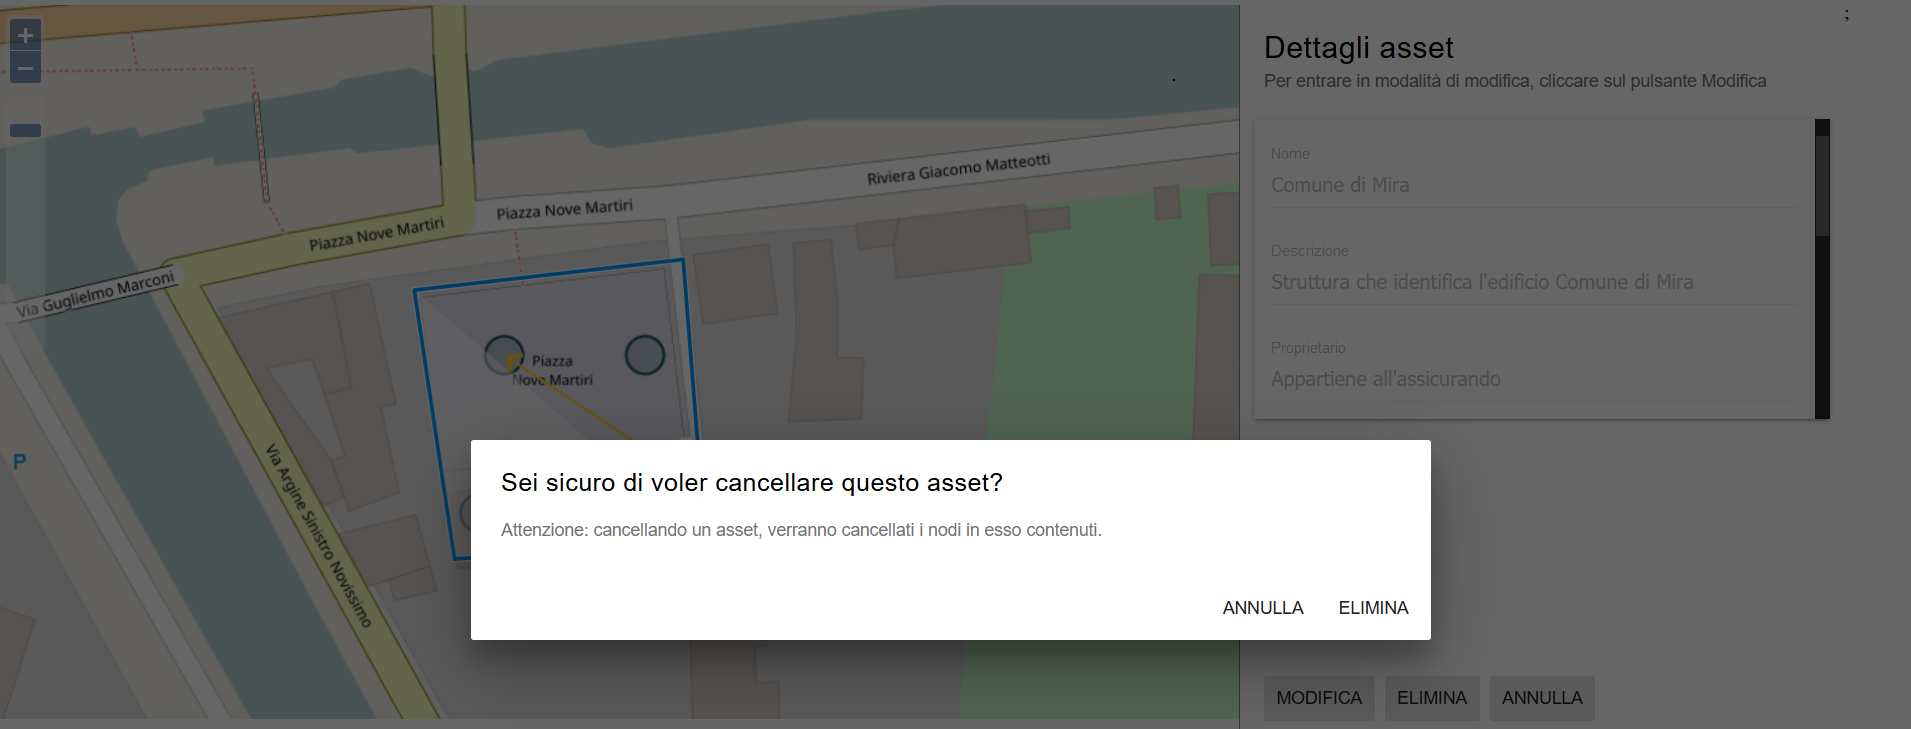
\includegraphics[width=\textwidth]{img/eliminazione_bloccante_asset.png}
\caption{Eliminazione di un asset}
\end{figure}
\section{Gestione nodo}
Per quanto riguarda la gestione dei nodi l'utente ha la possibilità di:
\begin{itemize}
	\item aggiungere un \mglo{Nodo}{nodo};
	\item visualizzare i dettagli relativi a un certo nodo presente;
	\item modificare un nodo presente;
	\item eliminare un nodo presente.
\end{itemize}

\subsection{Aggiunta di un nodo}
Per aggiungere un nodo si deve:
\begin{itemize}
	\item cliccare sul pulsante "+" in basso a destra della mappa;
	\item selezionare la voce "Aggiungi nodo";
	\item posizionare il nodo sulla mappa all'interno di un \mglo{Asset}{asset};
	\item compilare i campi (tutti) rispettando i vincoli esposti nell'apposita appendice \nameref{Validazioni};
	\item cliccare sul pulsante "Salva", che verrà abilitato solo nel momento in cui tutte le operazioni sopra descritte sono state eseguite in maniera corretta.
\end{itemize}

\begin{figure}[H]
\centering
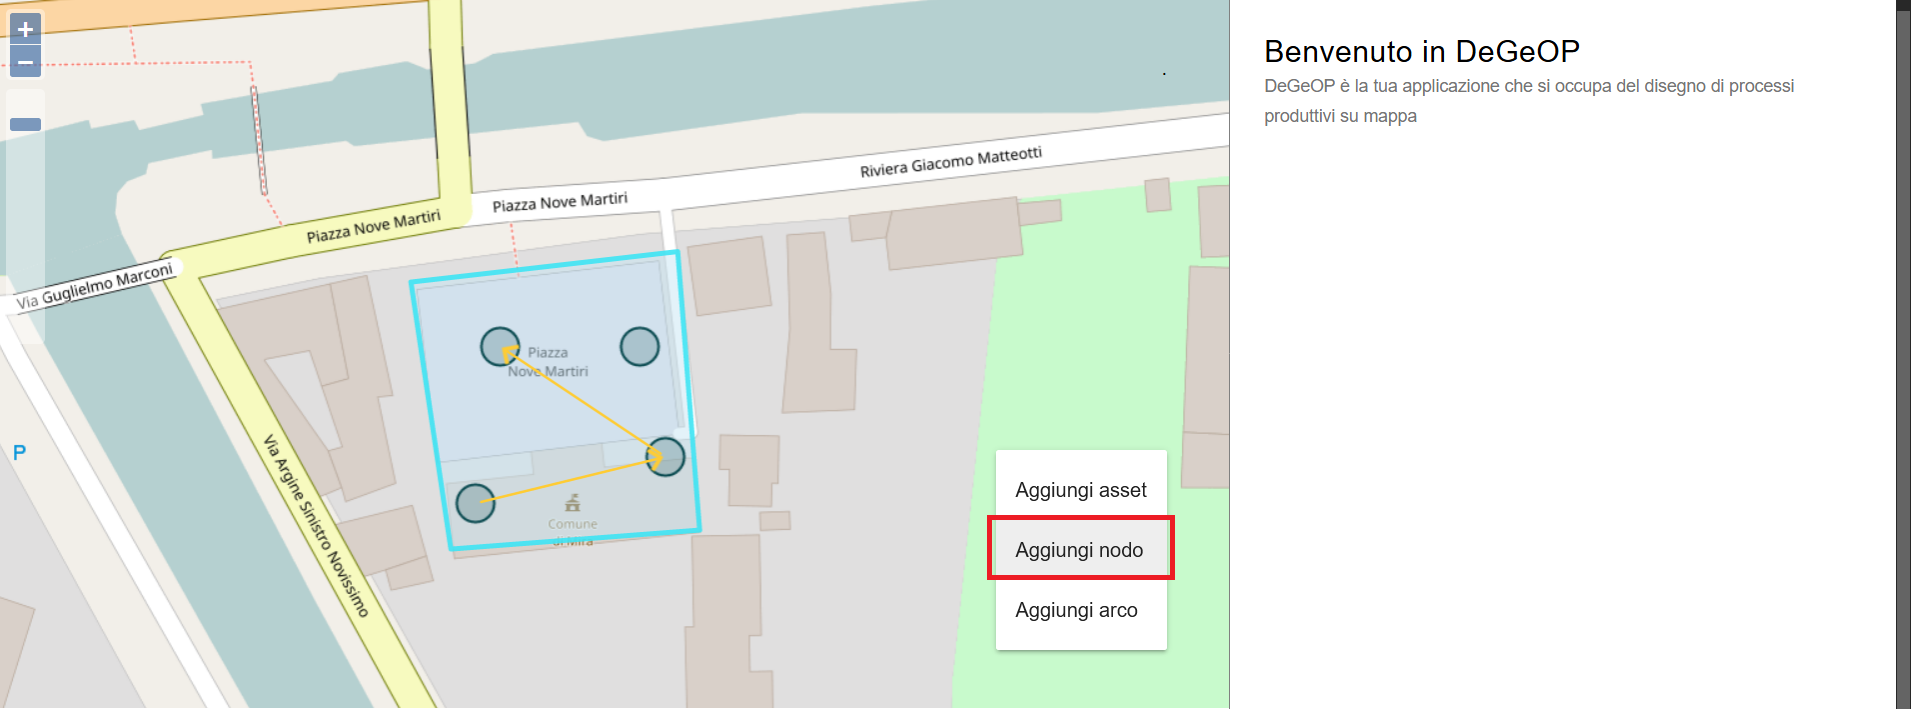
\includegraphics[width=\textwidth]{img/menu_aperto_nodo_hover.png}
\caption{Menu di aggiunta}
\end{figure}

\begin{figure}[H]
\centering
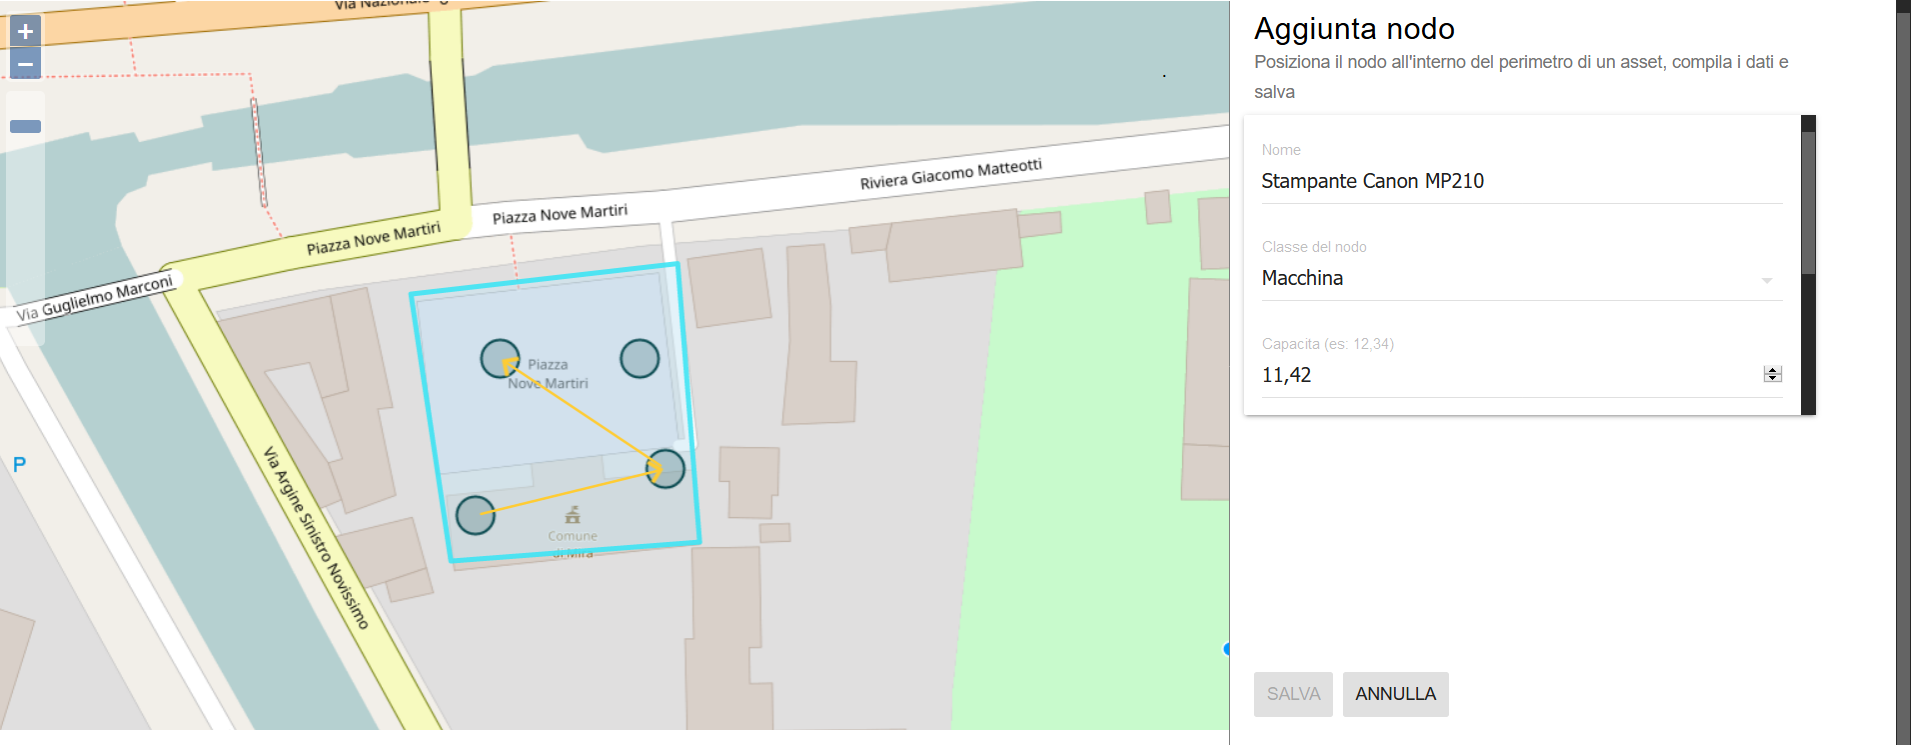
\includegraphics[width=\textwidth]{img/aggiunta_nodo.png}
\caption{Aggiunta di un nodo}
\end{figure}

\subsection{Visualizzazione dei dettagli di un nodo}
Per visualizzare i dettagli di un nodo si deve:
\begin{itemize}
	\item selezionare il  nodo che si intende modificare cliccando direttamente su quel nodo dalla mappa.
\end{itemize}

\begin{figure}[H]
\centering
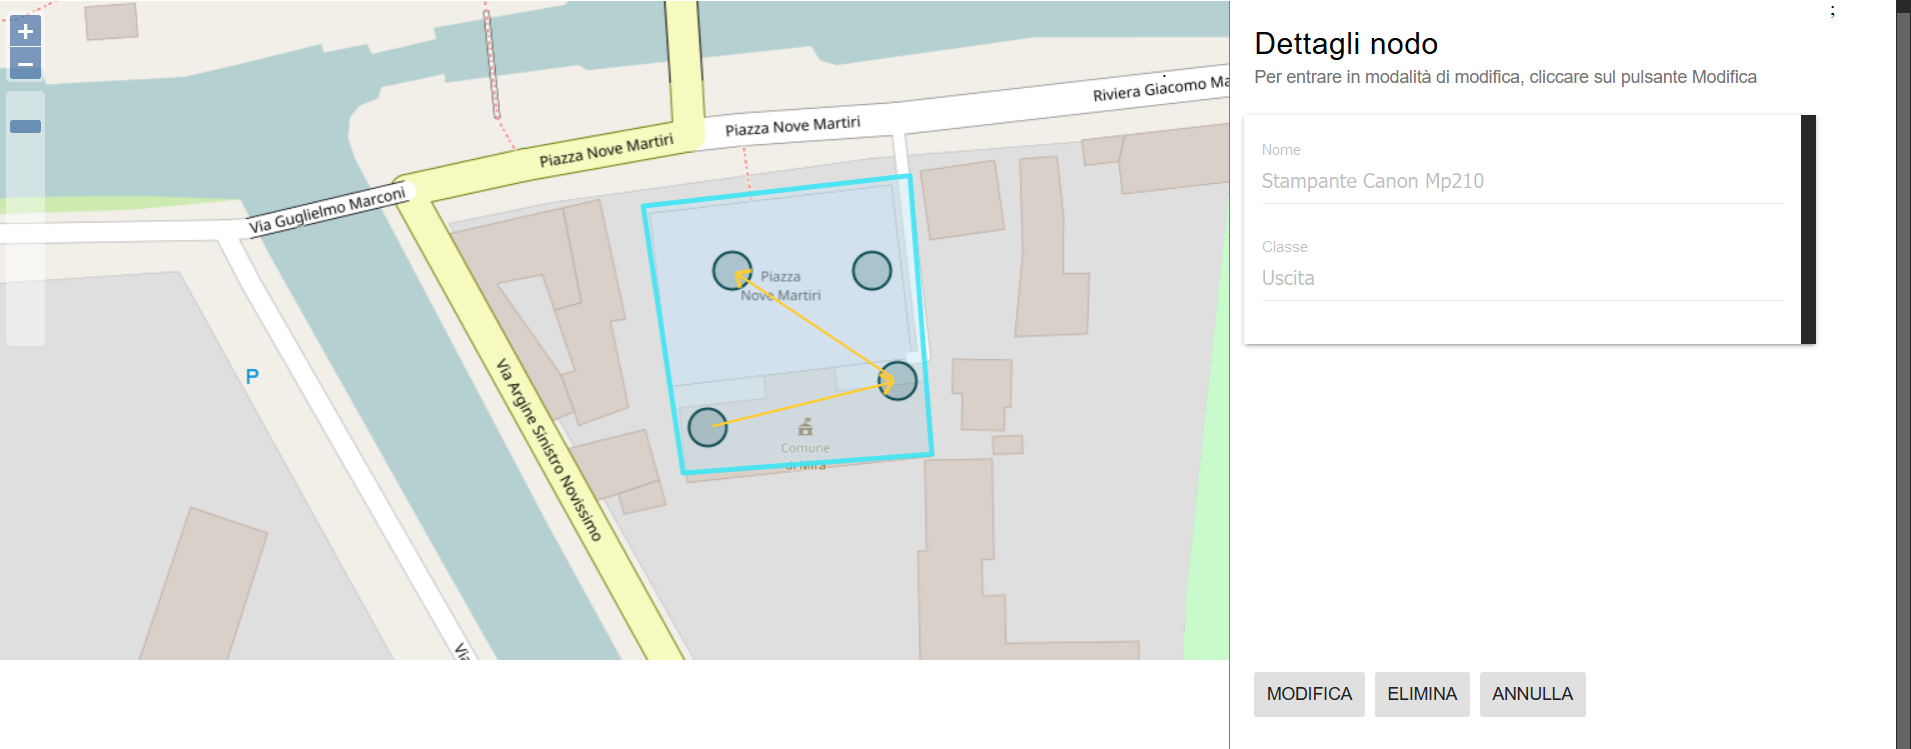
\includegraphics[width=\textwidth]{img/visualizzazione_nodo.png}
\caption{Visualizzazione dettagli di un nodo}
\end{figure}

\subsection{Modifica di un nodo}
Per modificare un nodo si deve:
\begin{itemize}
	\item selezionare il nodo che si intende modificare cliccando direttamente sulla mappa;
	\item cliccare sul pulsante "Modifica" in basso sulla sidebar;
	\item eventualmente riposizionare il perimetro del nodo sulla mappa all'interno di un certo asset. La nuova posizione andrà in automatico a sovrascrivere quello precedentemente presente.
	\item eventualmente modificare i campi rispettando i vincoli esposti nell'apposita appendice \nameref{Validazioni};
	\item cliccare sul pulsante "Salva", che verrà abilitato solo nel momento in cui tutte le operazioni sopra descritte sono state eseguite in maniera corretta.
\end{itemize}

\begin{figure}[H]
\centering
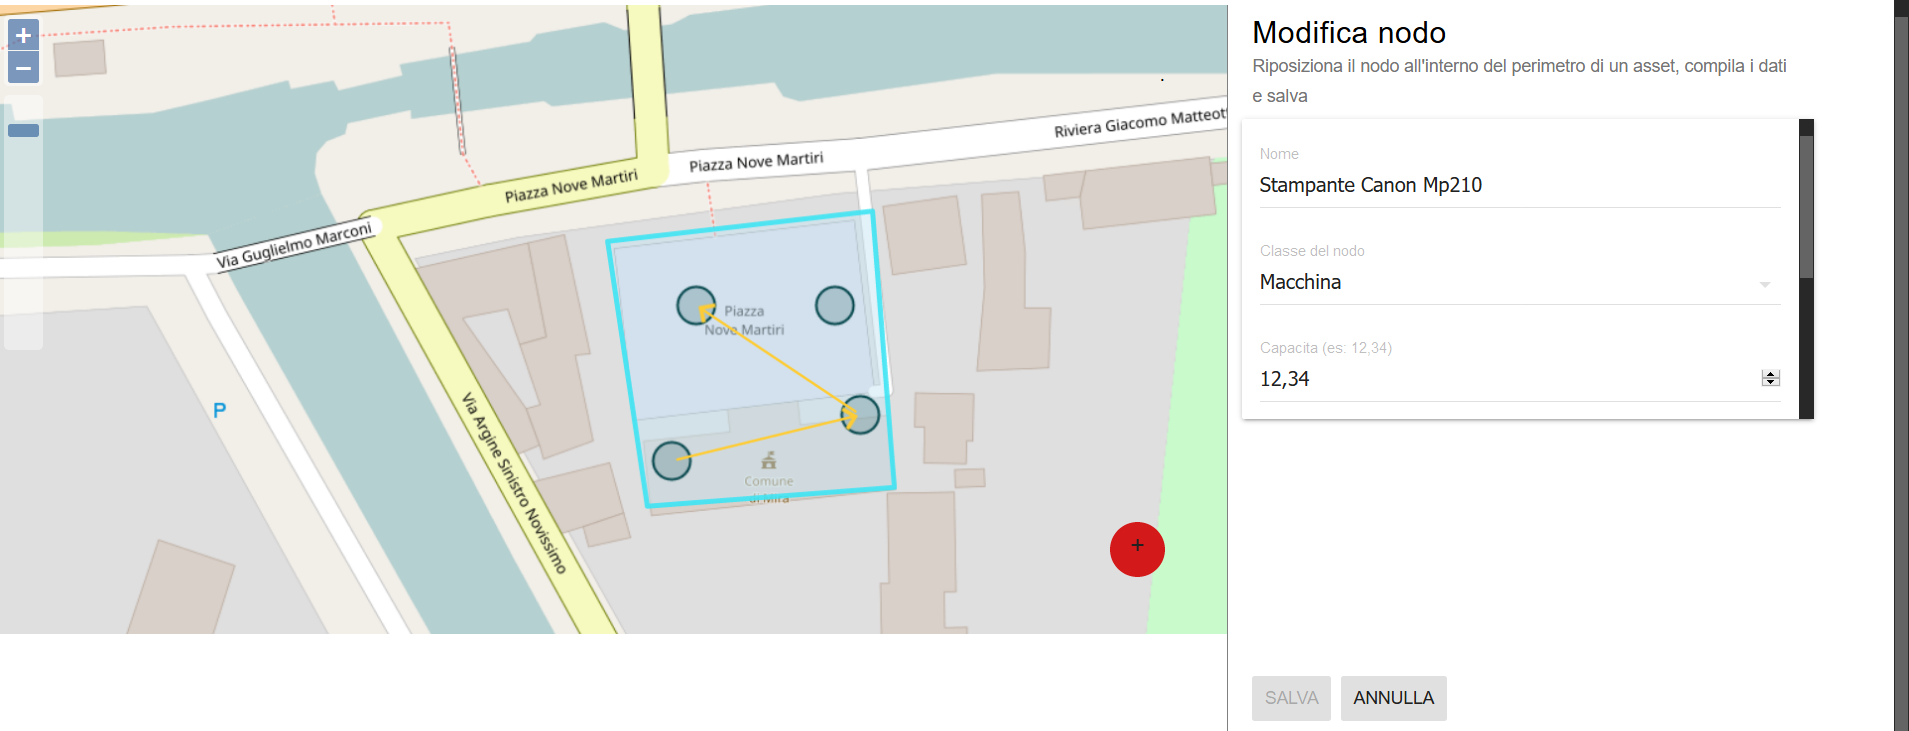
\includegraphics[width=\textwidth]{img/modifica_nodo.png}
\caption{Modifica di un nodo}
\end{figure}

\subsection{Eliminazione di un nodo}
Per eliminare un nodo si deve:
\begin{itemize}
	\item selezionare  nodo che si intende modificare cliccando direttamente sulla mappa;
	\item cliccare sul pulsante "Elimina" in basso sulla sidebar;
	\item cliccare sul pulsante "Elimina" sulla finestra bloccante che compare.
\end{itemize}

\begin{figure}[H]
\centering
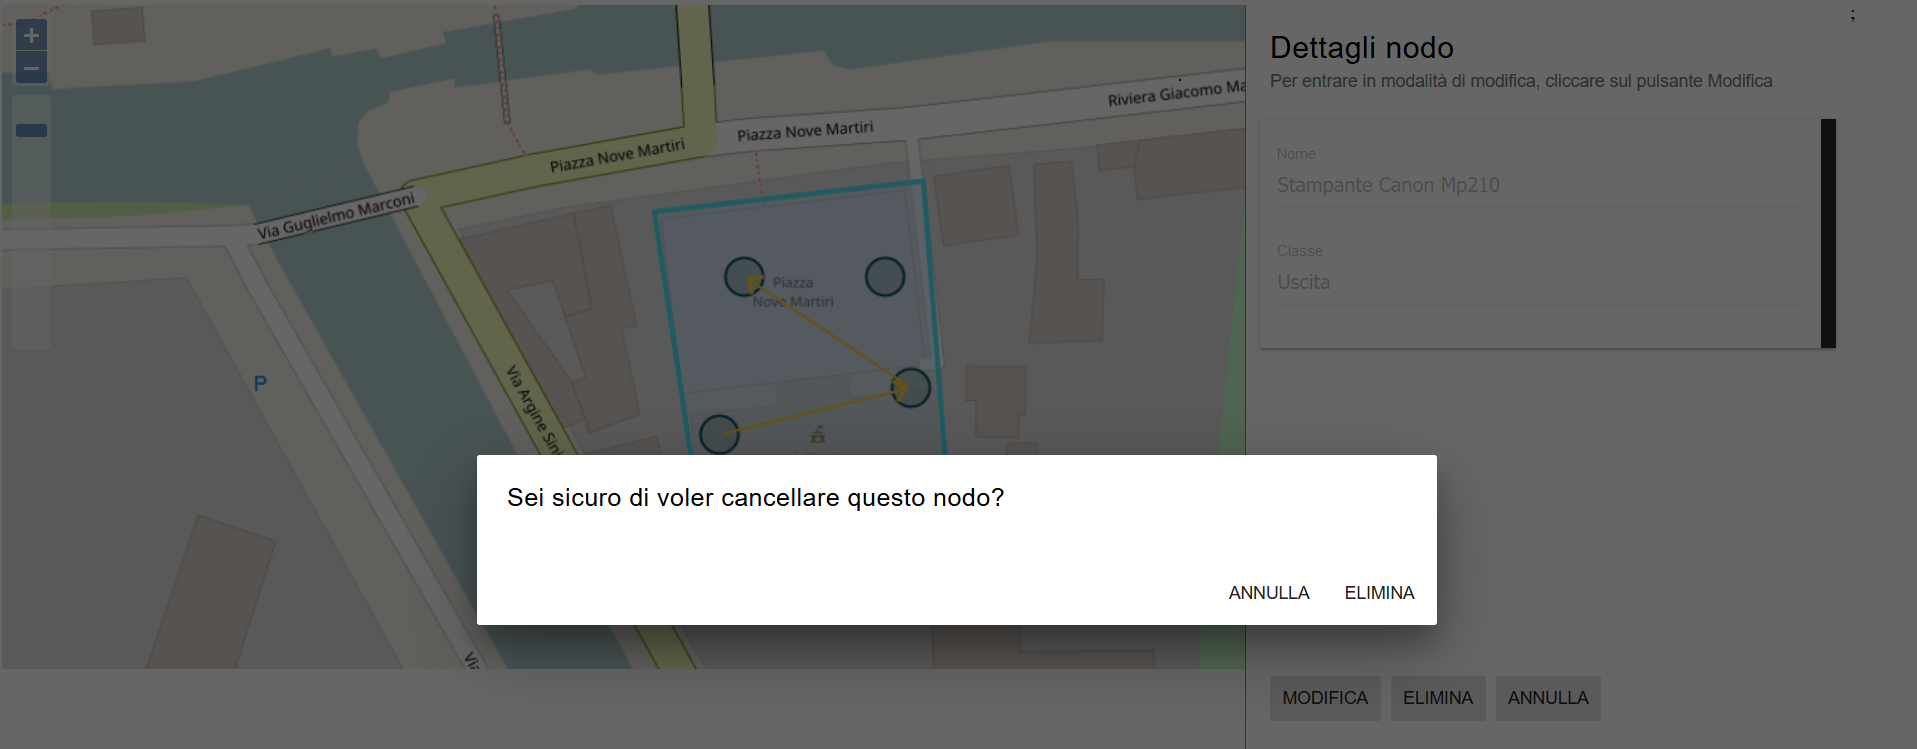
\includegraphics[width=\textwidth]{img/eliminazione_bloccante_nodo.png}
\caption{Eliminazione di un nodo}
\end{figure}
\section{Gestione arco}
Per quanto riguarda la gestione degli archi, l'utente ha la possibilità di:
\begin{itemize}
	\item aggiungere un \mglo{Arco}{arco};
	\item visualizzare i dettagli relativi a un certo arco presente;
	\item modificare un arco presente;
	\item eliminare un arco presente;
\end{itemize}

\subsection{Aggiunta di un arco}
Per aggiungere un arco si deve:
\begin{itemize}
	\item cliccare sul pulsante "+" in basso a destra della mappa;
	\item selezionare la voce "Aggiungi arco";
	\item selezionare il nodo di inizio e il \mglo{Nodo}{nodo} di fine sulla mappa;
	\item cliccare sul pulsante "Salva", che verrà abilitato solo nel momento in cui tutte le operazioni sopra descritte sono state eseguite in maniera corretta.
\end{itemize}

\begin{figure}[H]
\centering
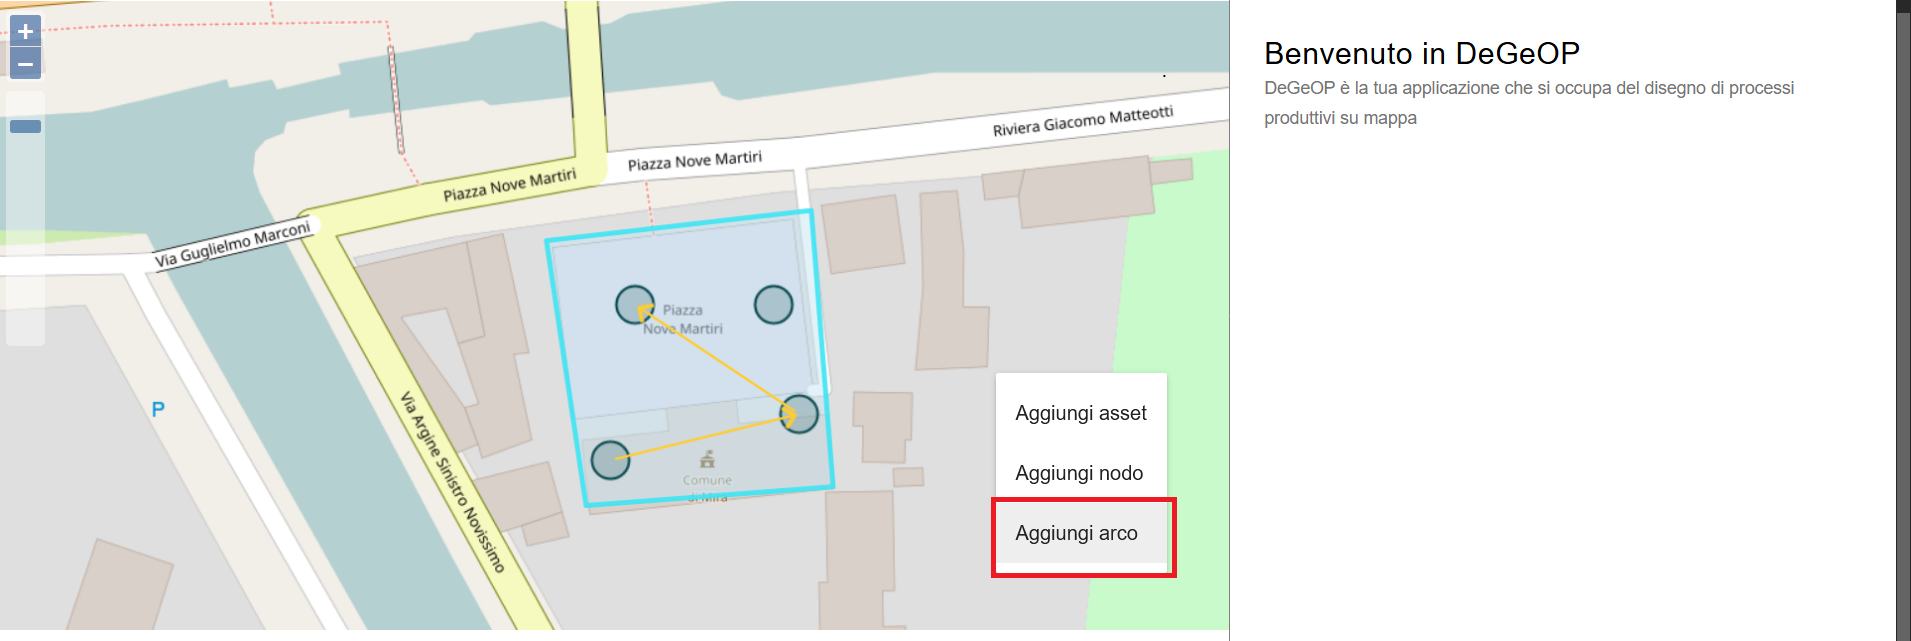
\includegraphics[width=\textwidth]{img/menu_aperto_arco_hover.png}
\caption{Menu di aggiunta}
\end{figure}

\begin{figure}[H]
\centering
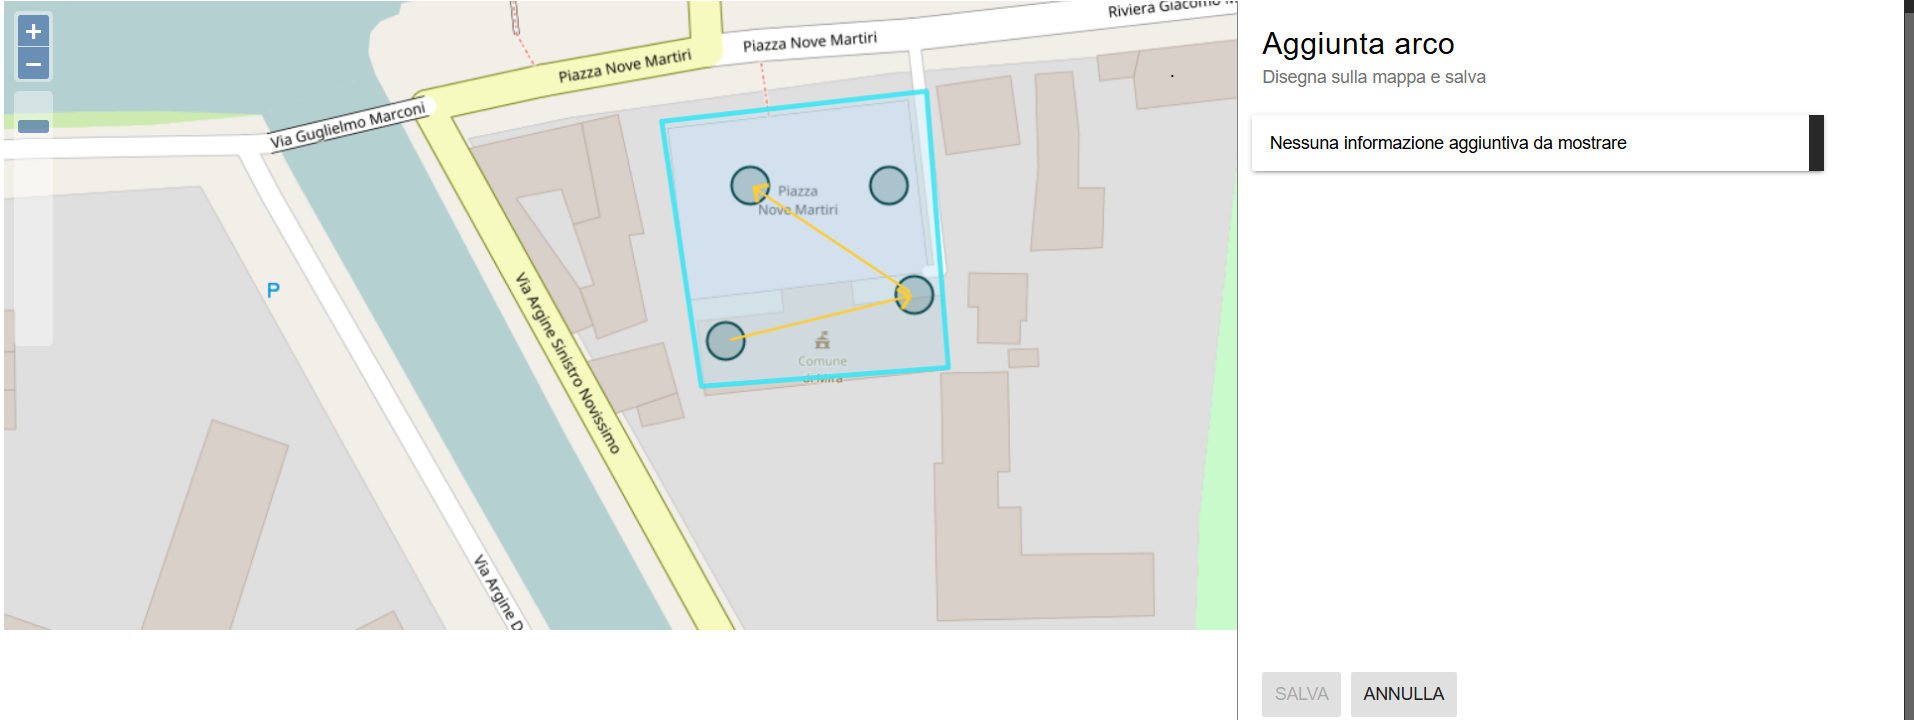
\includegraphics[width=\textwidth]{img/aggiunta_arco.png}
\caption{Aggiunta di un arco}
\end{figure}

\subsection{Visualizzazione dei dettagli di un arco}
Per visualizzare i dettagli di un arco si deve:
\begin{itemize}
	\item selezionare l'arco che si intende modificare cliccando direttamente su quell'arco dalla mappa.
\end{itemize}

\begin{figure}[H]
\centering
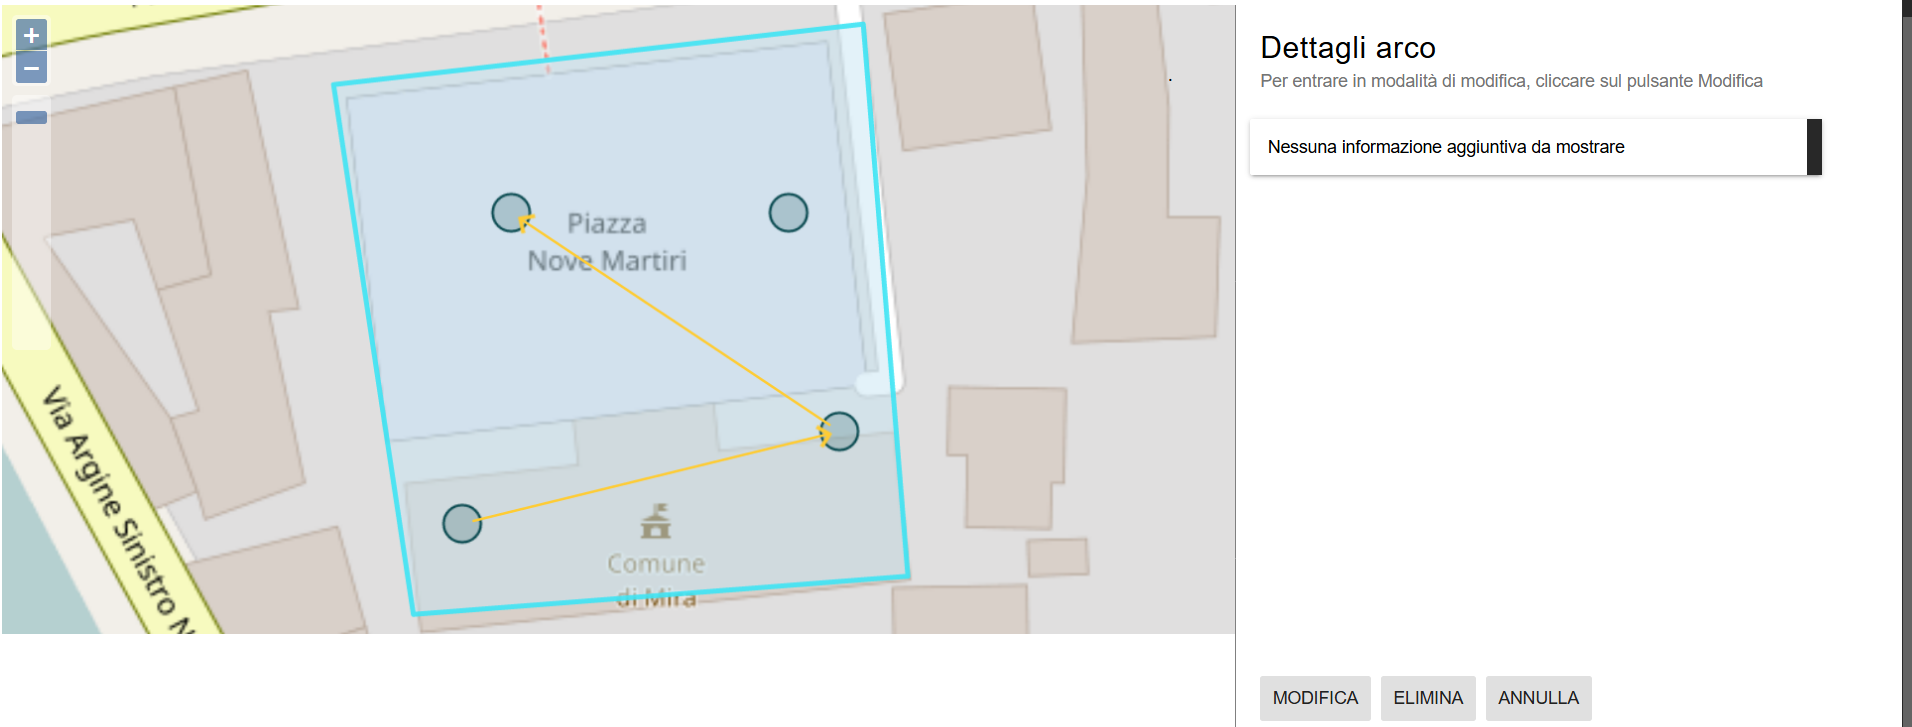
\includegraphics[width=\textwidth]{img/visualizzazione_arco.png}
\caption{Visualizzazione dettagli di un arco}
\end{figure}

\subsection{Modifica di un arco}
Per modificare un arco si deve:
\begin{itemize}
	\item selezionare l'arco che si intende modificare cliccando direttamente sulla mappa;
	\item cliccare sul pulsante "Modifica" in basso sulla sidebar;
	\item eventualmente selezionare il nodo di inizio e il nodo di fine sulla mappa. Il nuovo arco tracciato andrà in automatico a sovrascrivere quello precedentemente presente;
	\item cliccare sul pulsante "Salva", che verrà abilitato solo nel momento in cui tutte le operazioni sopra descritte sono state eseguite in maniera corretta.
\end{itemize}

\begin{figure}[H]
\centering
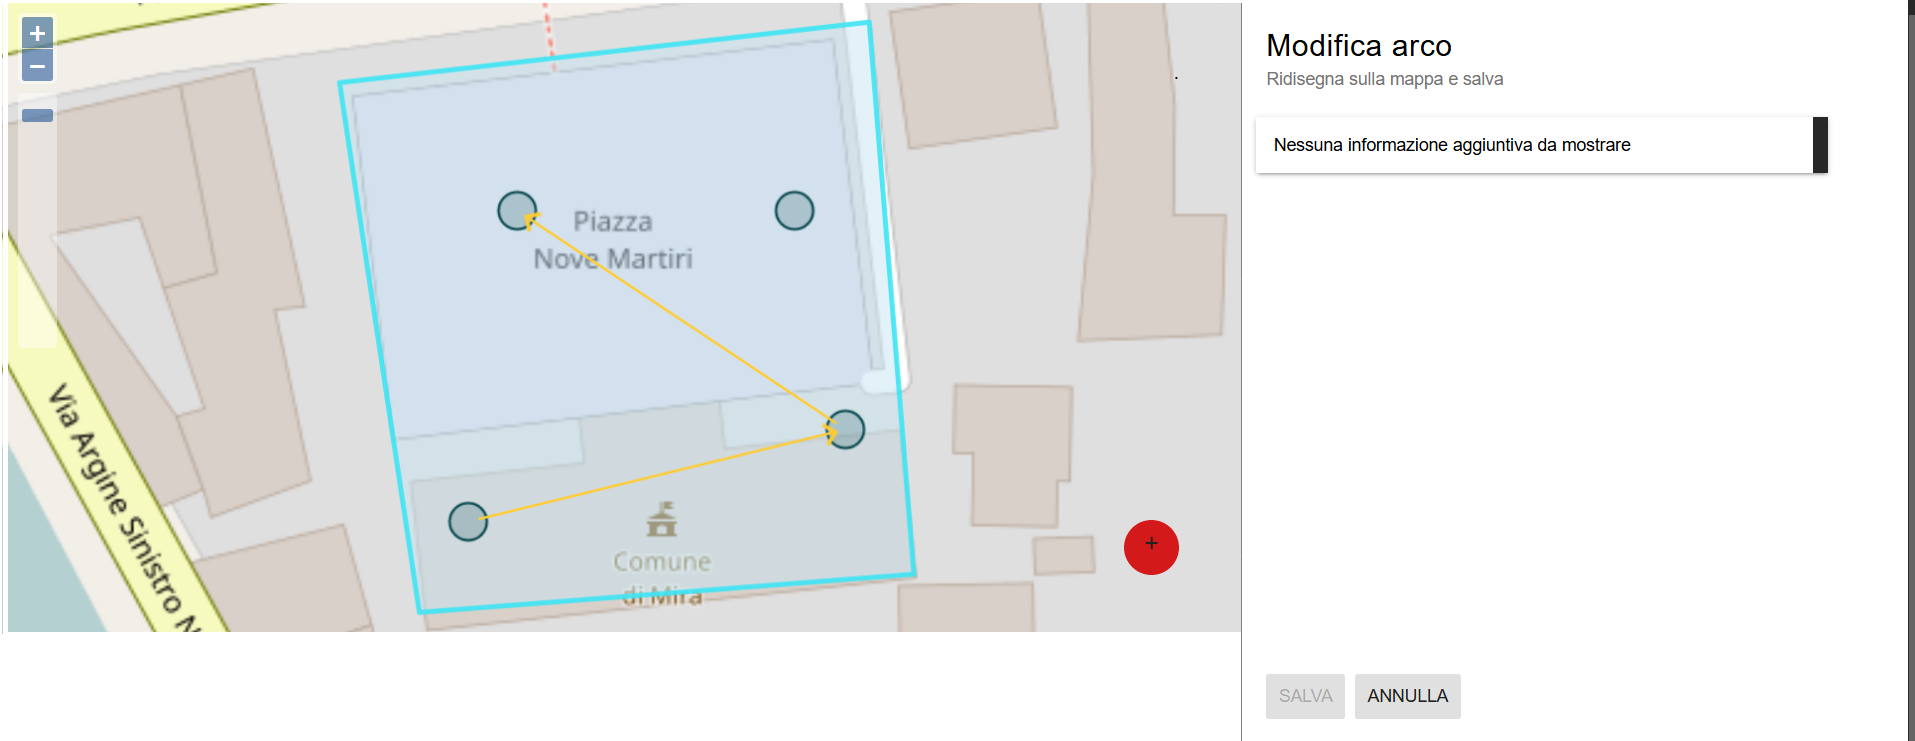
\includegraphics[width=\textwidth]{img/modifica_arco.png}
\caption{Modifica di un arco}
\end{figure}

\subsection{Eliminazione di un arco}
Per eliminare un arco si deve:
\begin{itemize}
	\item selezionare l'arco che si intende modificare cliccando direttamente sulla mappa;
	\item cliccare sul pulsante "Elimina" in basso sulla sidebar;
	\item cliccare sul pulsante "Elimina" sulla finestra bloccante che compare.
\end{itemize}

\begin{figure}[H]
\centering
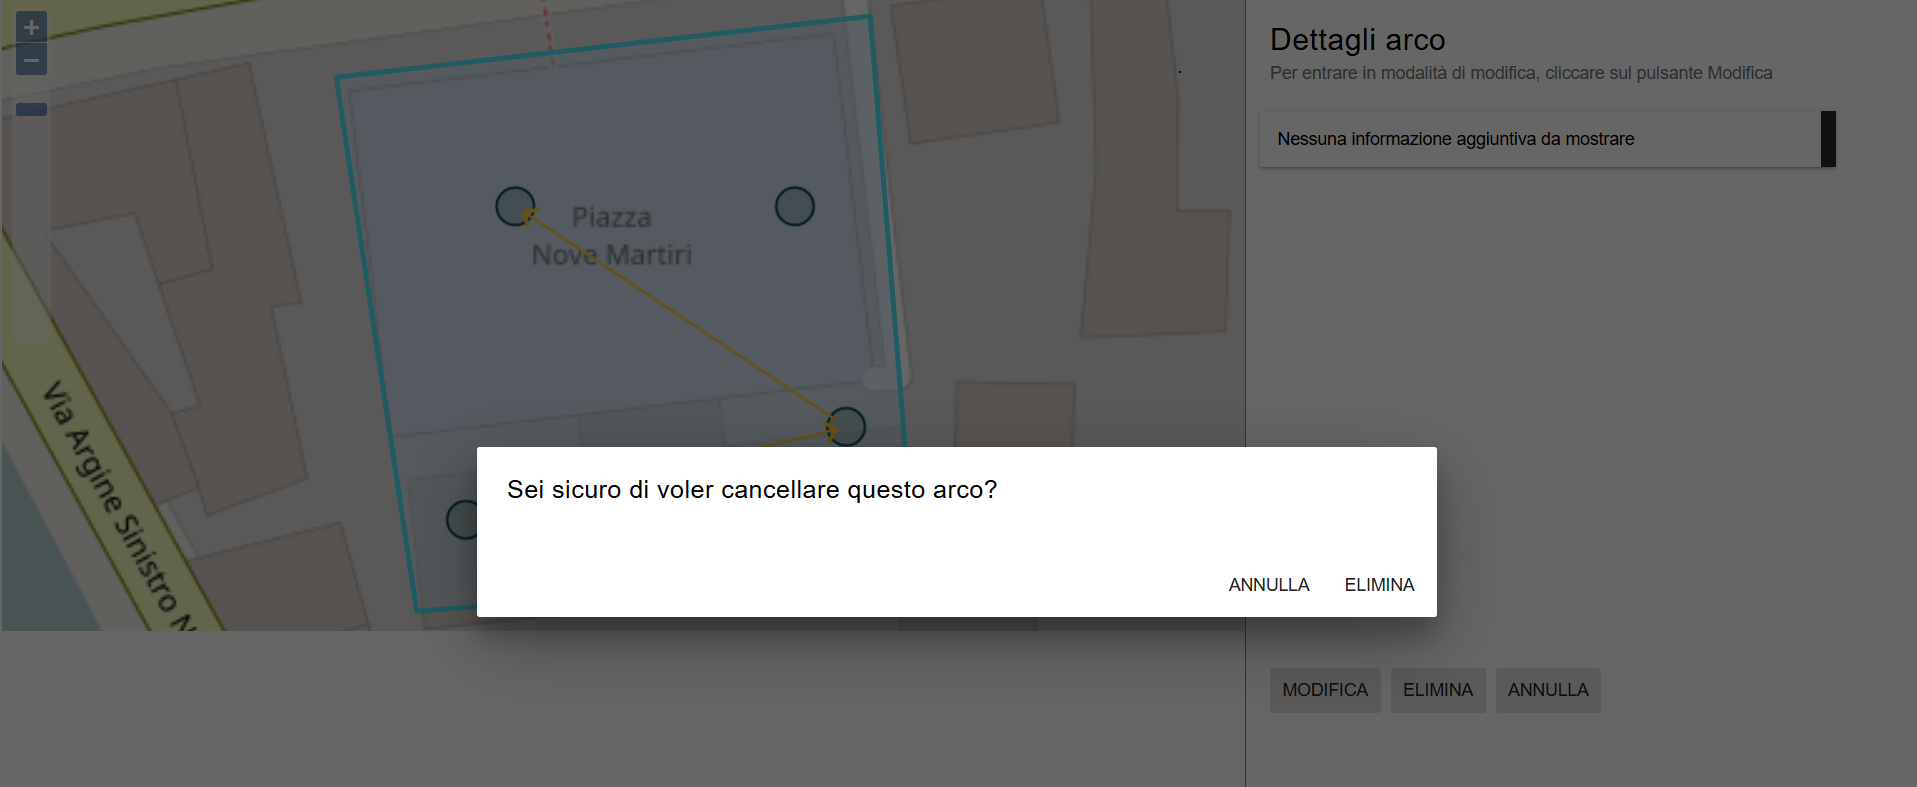
\includegraphics[width=\textwidth]{img/eliminazione_bloccante_arco.png}
\caption{Eliminazione di un arco}
\end{figure}
\section{Gestione scenario}
	Per quanto riguarda la gestione degli \mglo{Scenario}{scenario} l'utente ha la possibilità di:
	\begin{itemize}
		\item aggiungere uno scenario;
		\item visualizzare i dettagli relativi a un certo scenario presente;
		\item modificare uno scenario presente;
		\item eliminare uno scenario presente.
	\end{itemize}

\subsection{Aggiunta di uno scenario}
	Per aggiungere uno scenario si deve:
	\begin{itemize}
		\item cliccare sul pulsante "+" in basso a destra della mappa;
		\item selezionare la voce "Aggiungi scenario";
		\item disegnare il perimetro dello scenario sulla mappa. E' possibile apporre gli spigoli del perimetro cliccando direttamente sulla mappa. Il perimetro dello scenario deve essere correttamente chiuso, facendo coincidere l'ultimo spigolo del perimetro col primo;
		\item compilare i campi (tutti) rispettando i vincoli esposti nell'apposita appendice \nameref{Validazioni};
		\item cliccare sul pulsante "Salva", che verrà abilitato solo nel momento in cui tutte le operazioni sopra descritte sono state eseguite in maniera corretta.
	\end{itemize}
	
	\begin{figure}[H]
	\centering
	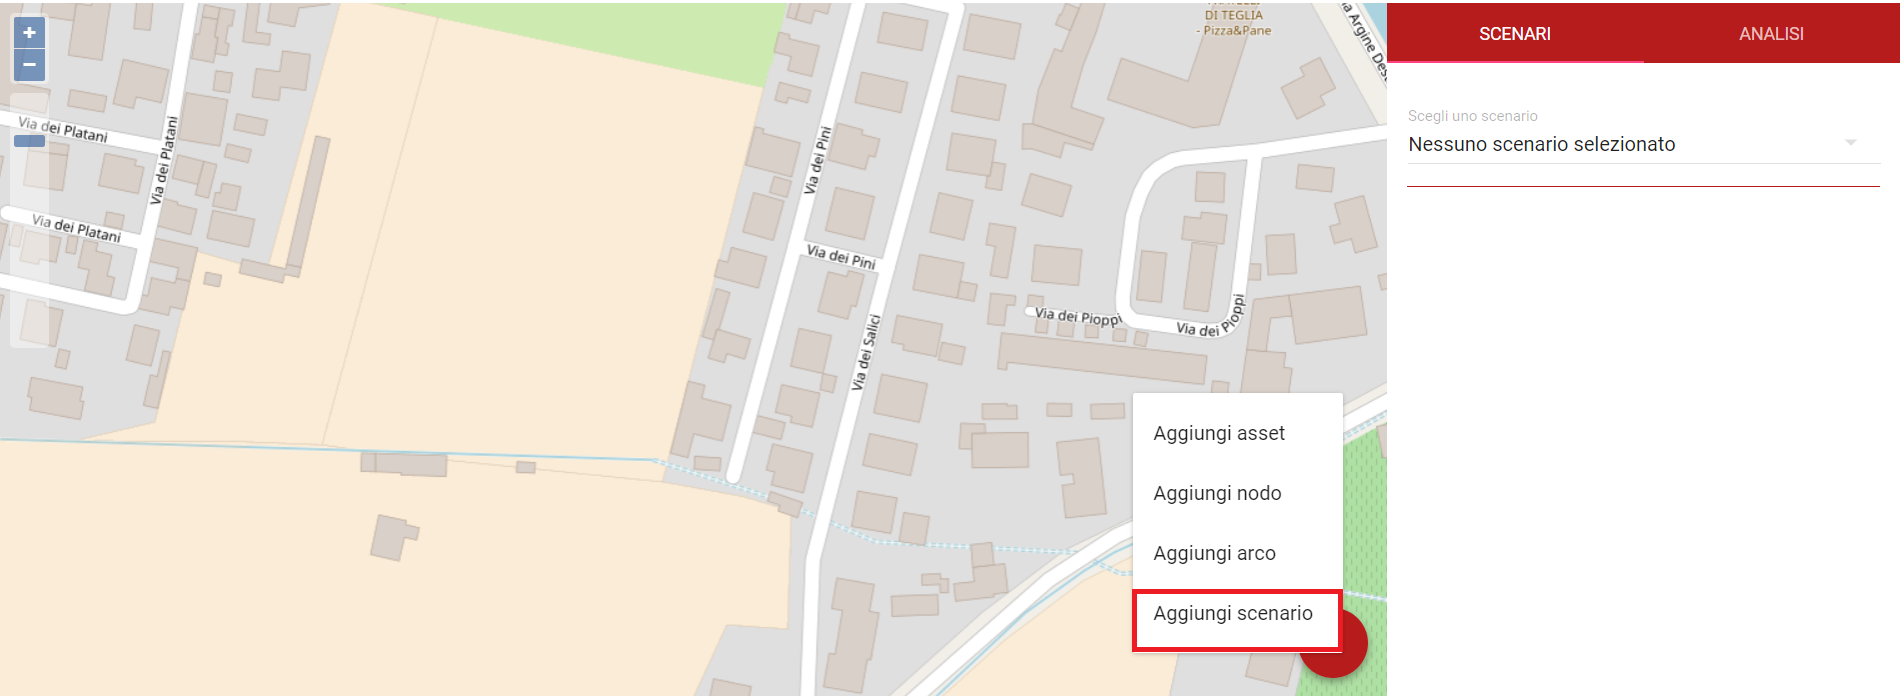
\includegraphics[width=\textwidth]{img/menu_aperto_scenario_hover.png}
	\caption{Menu di aggiunta}
	\end{figure}
	
	\begin{figure}[H]
	\centering
	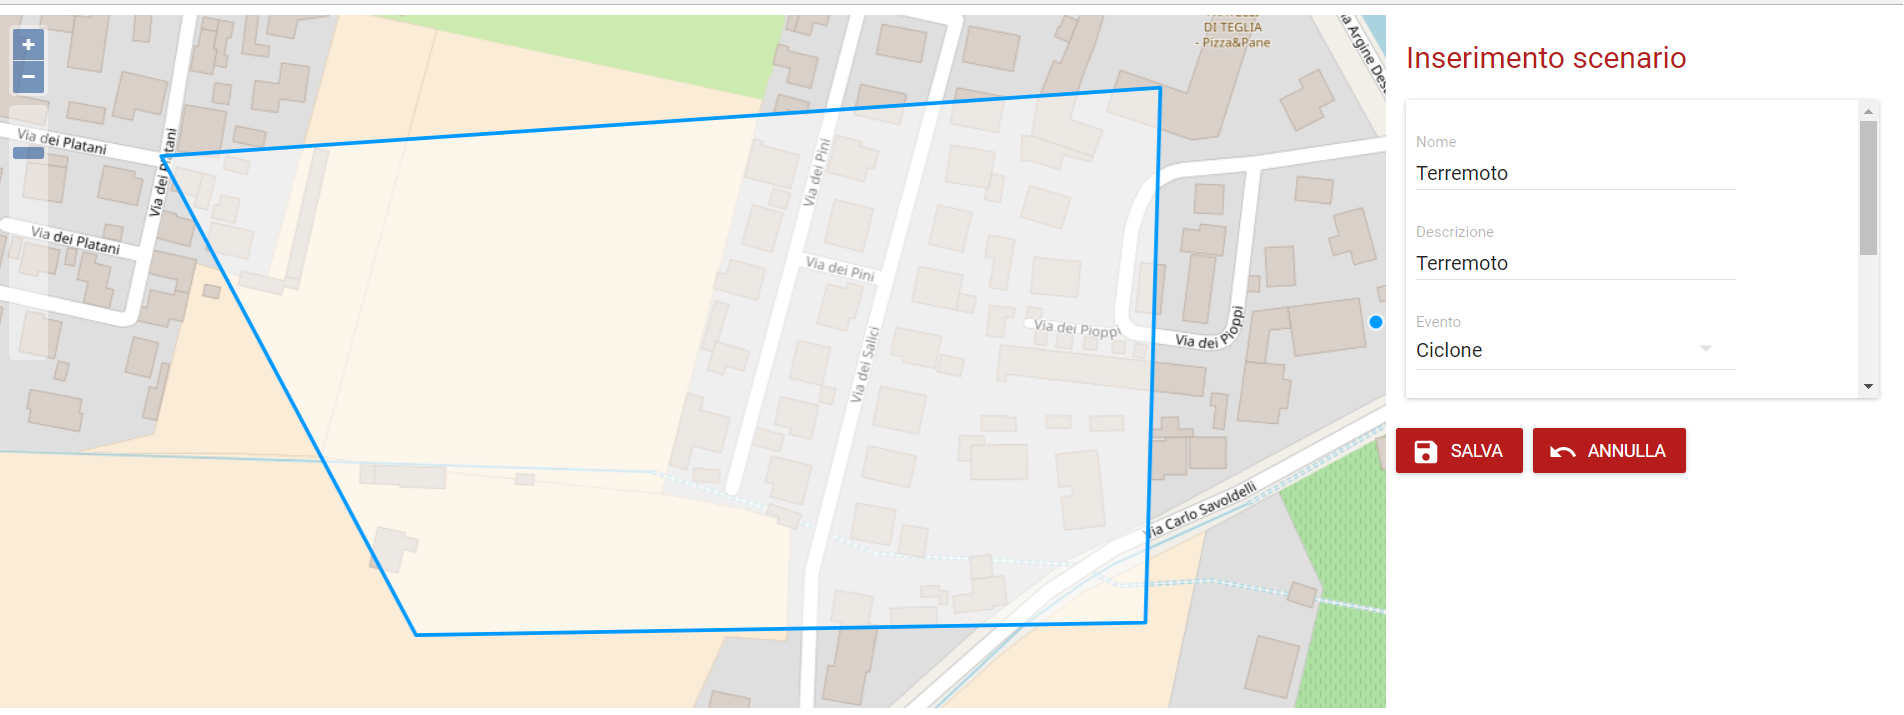
\includegraphics[width=\textwidth]{img/aggiunta_scenario.png}
	\caption{Aggiunta di uno scenario}
	\end{figure}

\subsection{Visualizzazione dei dettagli di uno scenario}
	Per visualizzare i dettagli di uno scenario si deve:
	\begin{itemize}
		\item selezionare l'scenario che si intende modificare cliccando direttamente su quell'scenario dalla mappa.
	\end{itemize}
	
	\begin{figure}[H]
	\centering
	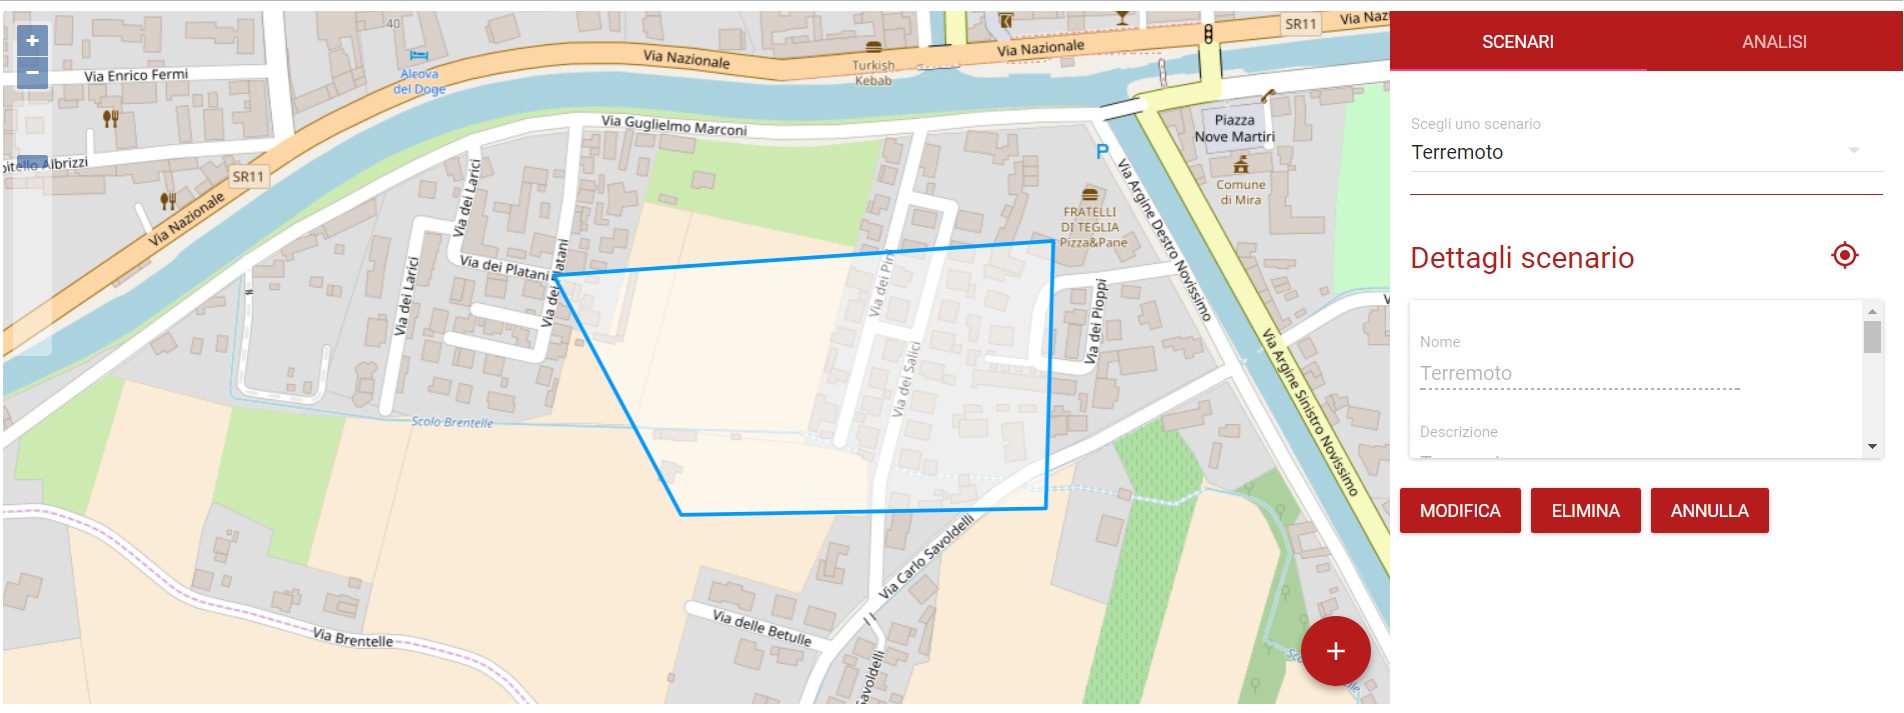
\includegraphics[width=\textwidth]{img/visualizzazione_scenario.png}
	\caption{Visualizzazione dettagli di uno scenario}
	\end{figure}

\subsection{Modifica di uno scenario}
	Per modificare uno scenario si deve:
	\begin{itemize}
		\item selezionare l'scenario che si intende modificare cliccando direttamente sulla mappa;
		\item cliccare sul pulsante "Modifica" in basso sulla sidebar;
		\item eventualmente ridisegnare il perimetro dello scenario sulla mappa. E' possibile apporre gli spigoli del perimetro cliccando direttamente sulla mappa. Il nuovo perimetro andrà in automatico a sovrascrivere quello precentemente presente. Il perimetro dello scenario deve essere correttamente chiuso, facendo coincidere l'ultimo spigolo del perimetro col primo;
		\item eventualmente modificare i campi rispettando i vincoli esposti nell'apposita appendice \nameref{Validazioni};
		\item cliccare sul pulsante "Salva", che verrà abilitato solo nel momento in cui tutte le operazioni sopra descritte sono state eseguite in maniera corretta.
	\end{itemize}
	
	\begin{figure}[H]
	\centering
	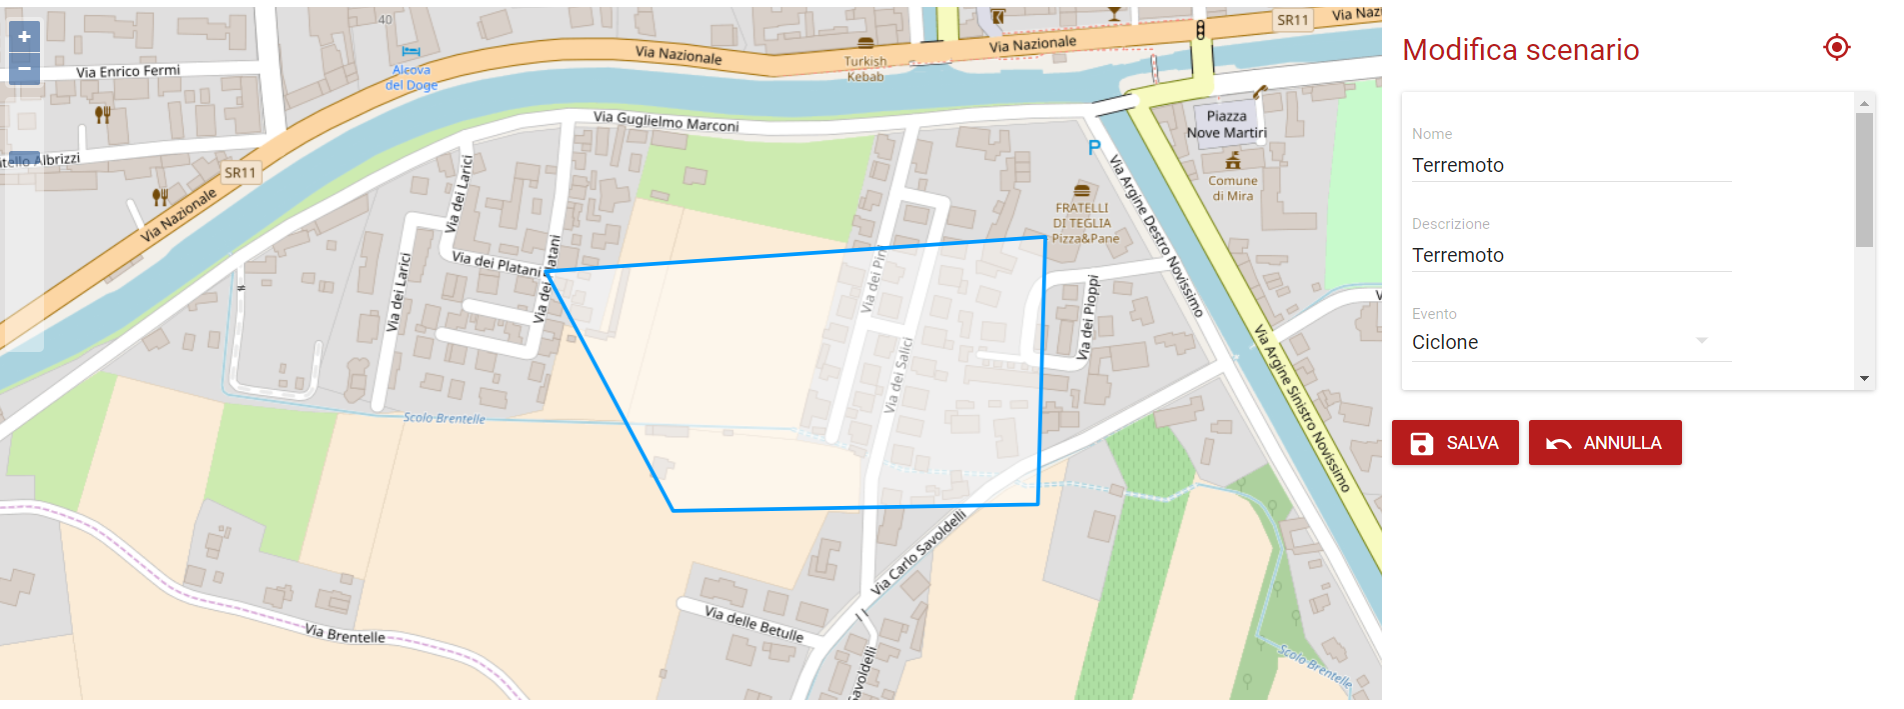
\includegraphics[width=\textwidth]{img/modifica_scenario.png}
	\caption{Modifica di uno scenario}
	\end{figure}

\subsection{Eliminazione di uno scenario}
Per eliminare uno scenario si deve:
\begin{itemize}
	\item selezionare l'scenario che si intende modificare cliccando direttamente sulla mappa;
	\item cliccare sul pulsante "Elimina" in basso sulla sidebar;
	\item cliccare sul pulsante "Elimina" sulla finestra bloccante che compare.
\end{itemize}

\begin{figure}[H]
\centering
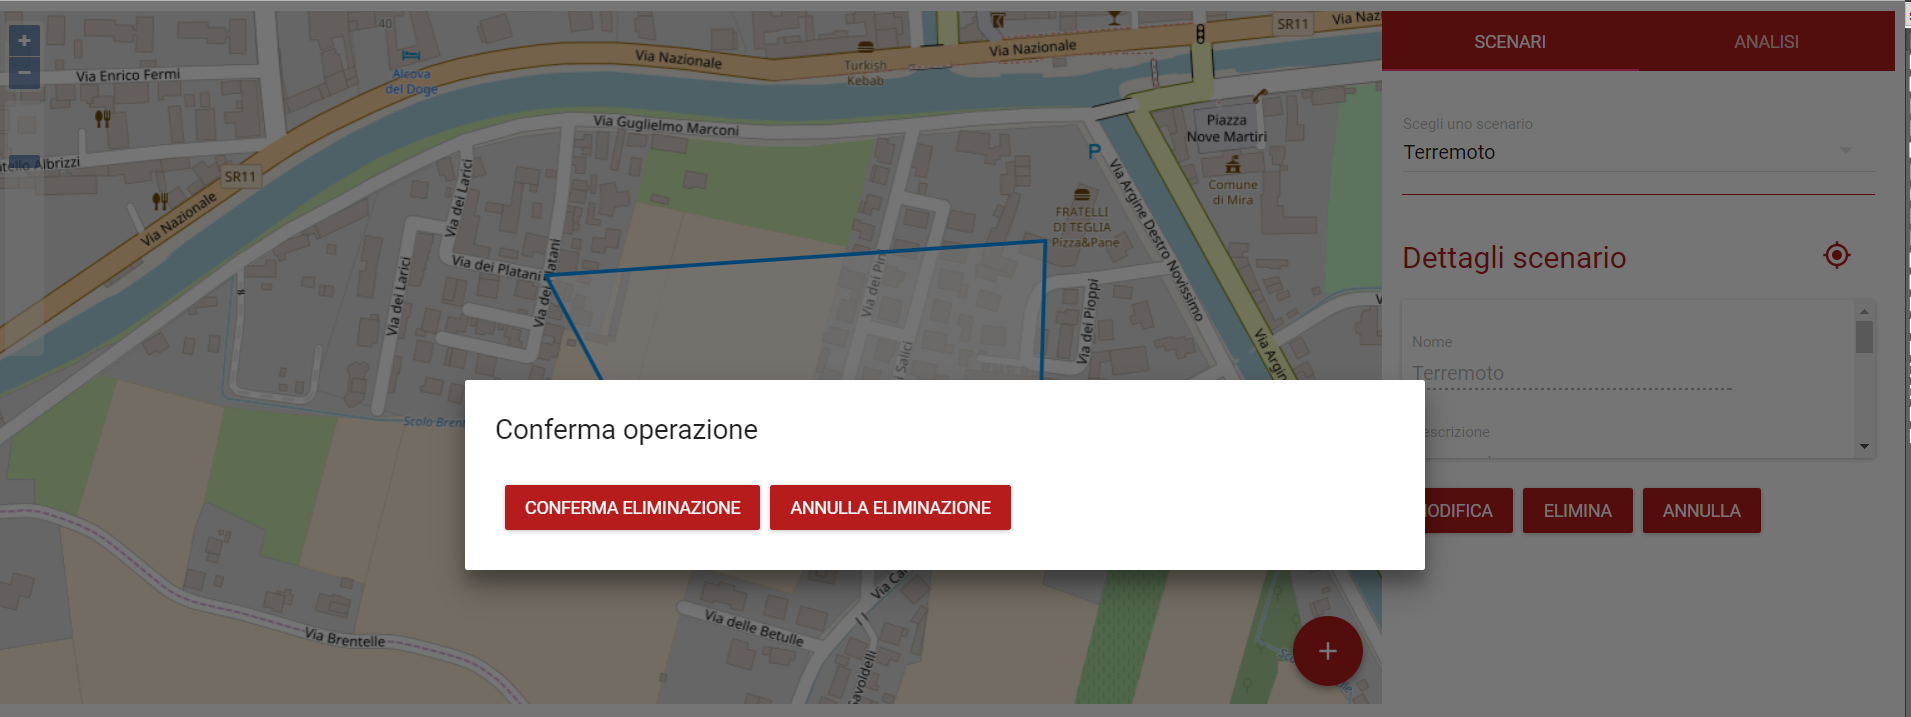
\includegraphics[width=\textwidth]{img/eliminazione_bloccante_scenario.png}
\caption{Eliminazione di uno scenario}
\end{figure}
\section{Gestione analisi}
	Per quanto riguarda la gestione delle \mglo{Analisi}{analisi}, l'utente ha la possibilità di:
	\begin{itemize}
		\item avviare un'analisi su certi scenari e visualizzare i risultati dell'analisi (sia in forma testuale sia su mappa) relativi agli scenari precedentemente scelti;
		\item cambiare l'anno di riferimento dei risultati di analisi (dopo 1, 2, o 3 anni) visualizzando i risultati dell'analisi aggiornati;
		\item cancellare risultati di analisi relativi a certi scenari su cui è stata calcolata una analisi.
	\end{itemize}
	
		\begin{figure}[H]
			\centering
			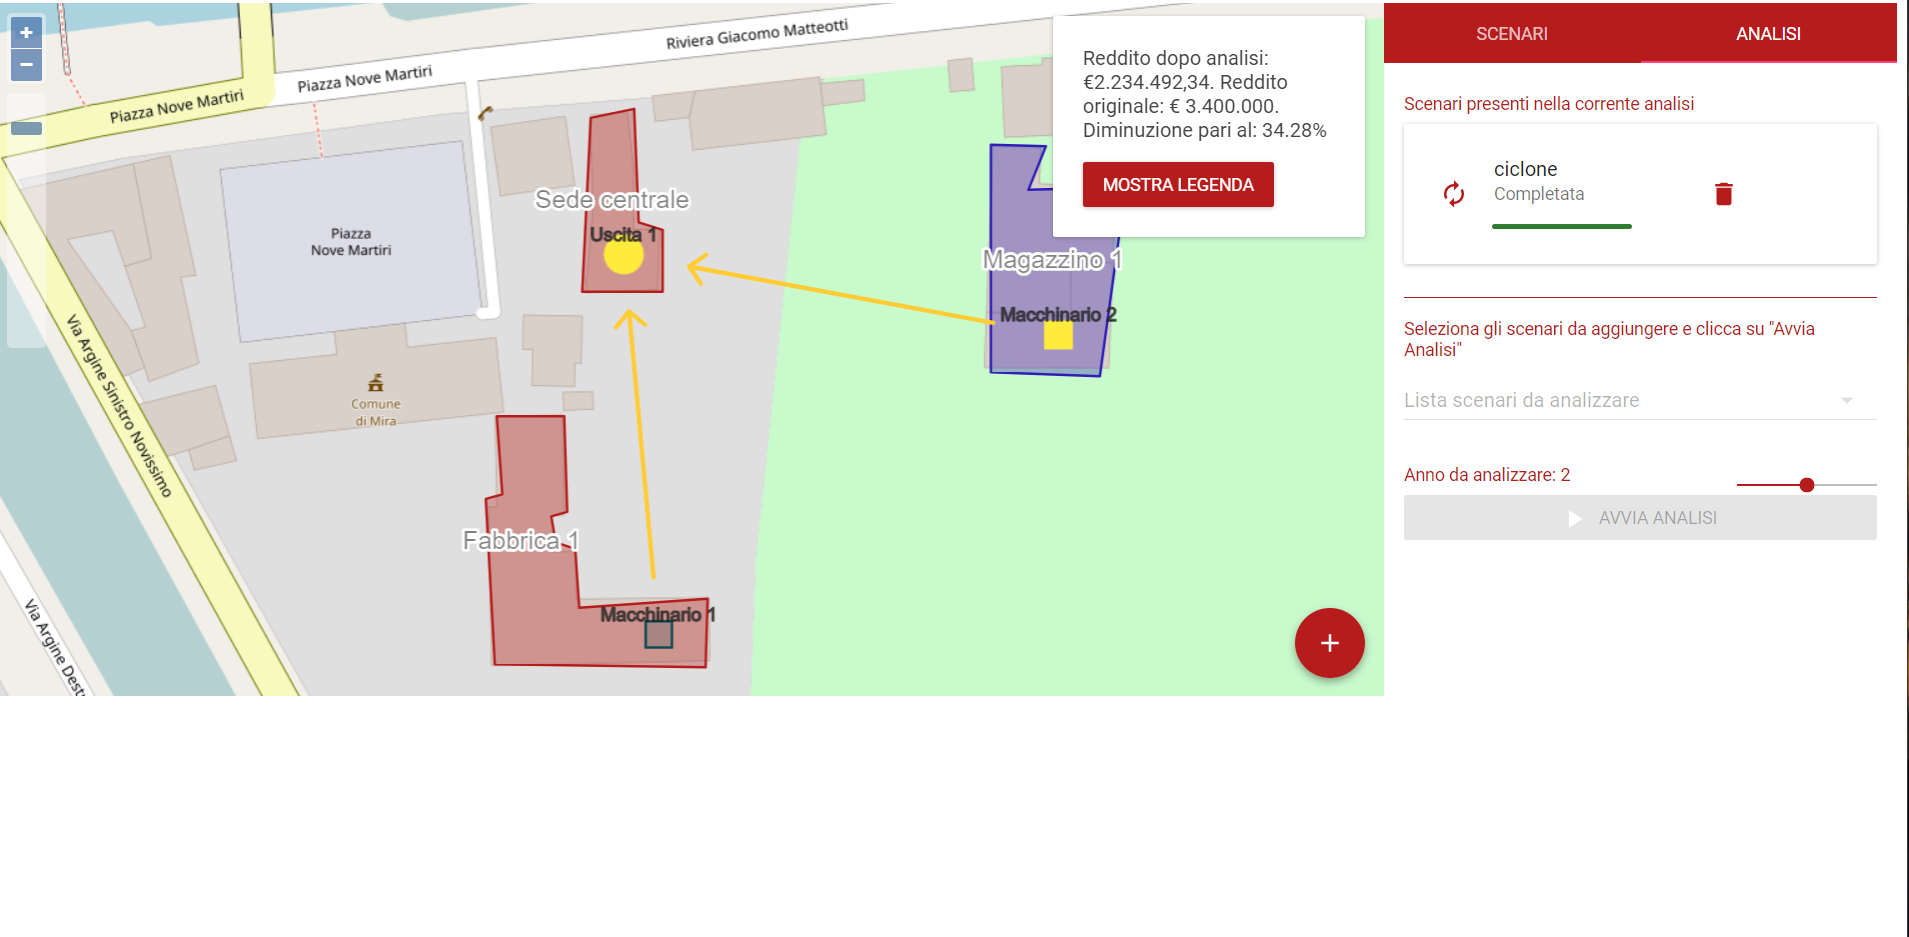
\includegraphics[width=\textwidth]{img/analisi.png}
			\caption{Menu di aggiunta}
		\end{figure}
		
\subsection{Avvio dell'analisi}
	Per avviare un'analisi di danno si deve:
	\begin{itemize}
		\item cliccare sulla lista di scenari da analizzare nella sidebar;
		\item selezionare uno o più scenari dal menù a tendina che si sarà aperto;
		\item premere sul pulsante "Avvia analisi".
	\end{itemize}

	\begin{figure}[H]
		\centering
		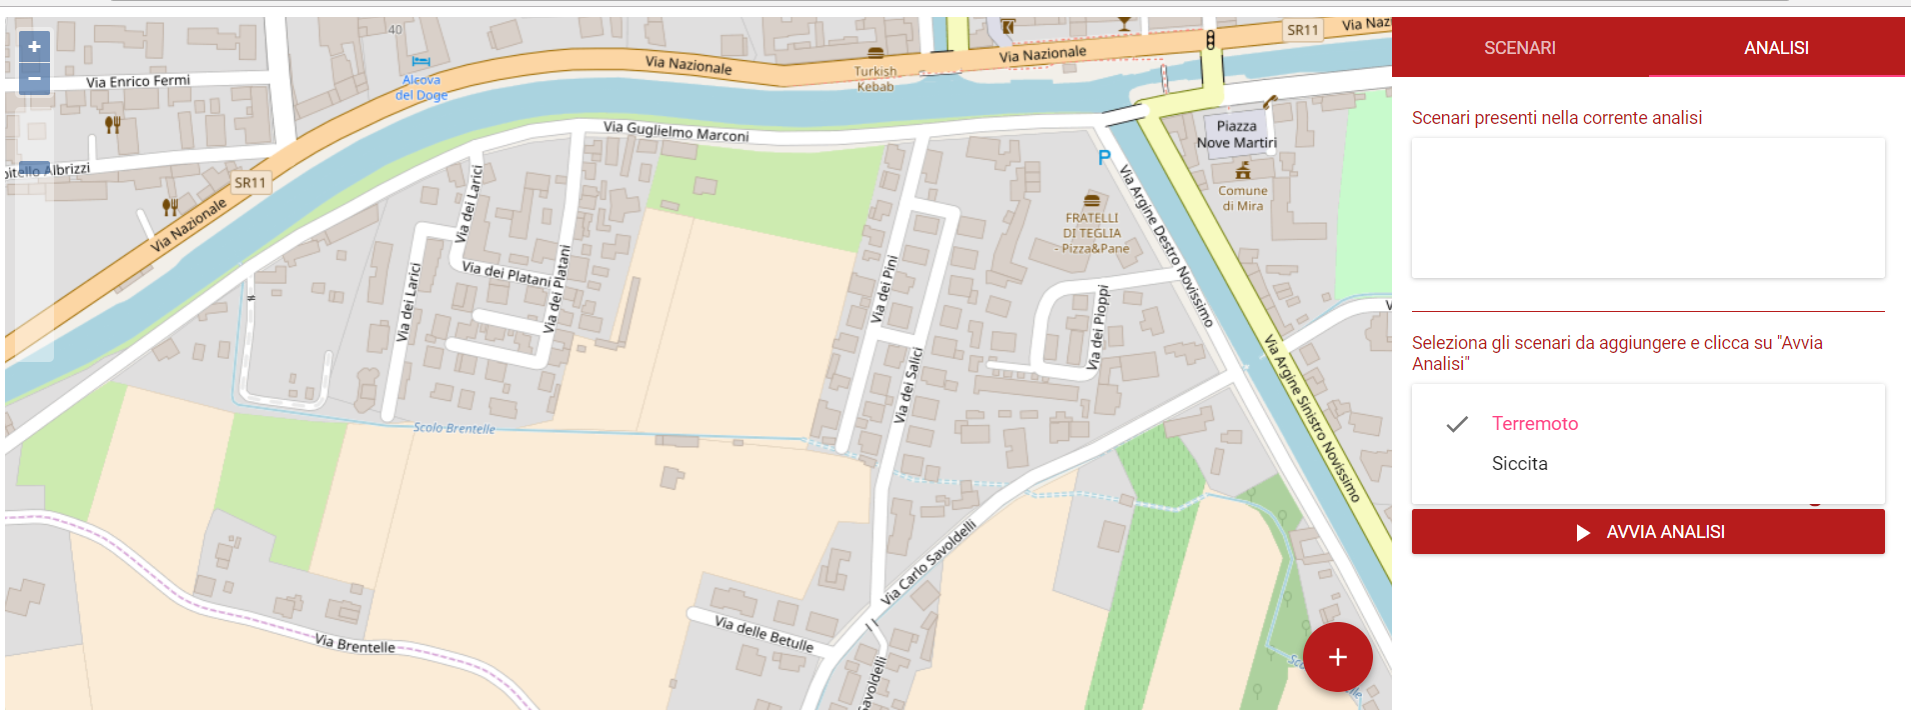
\includegraphics[width=\textwidth]{img/avvio_analisi.png}
		\caption{Avvio dell'analisi}
	\end{figure}

\subsection{Avanzamento analisi}
	Una volta avviata un'analisi, i suoi risultati non sono immediatamente disponibili, dato che è necessario del tempo per portare a termine il calcolo. L'avanzamento di questa operazione è visualizzato dalla barra presente nella sidebar.
	
	\begin{figure}[H]
		\centering
		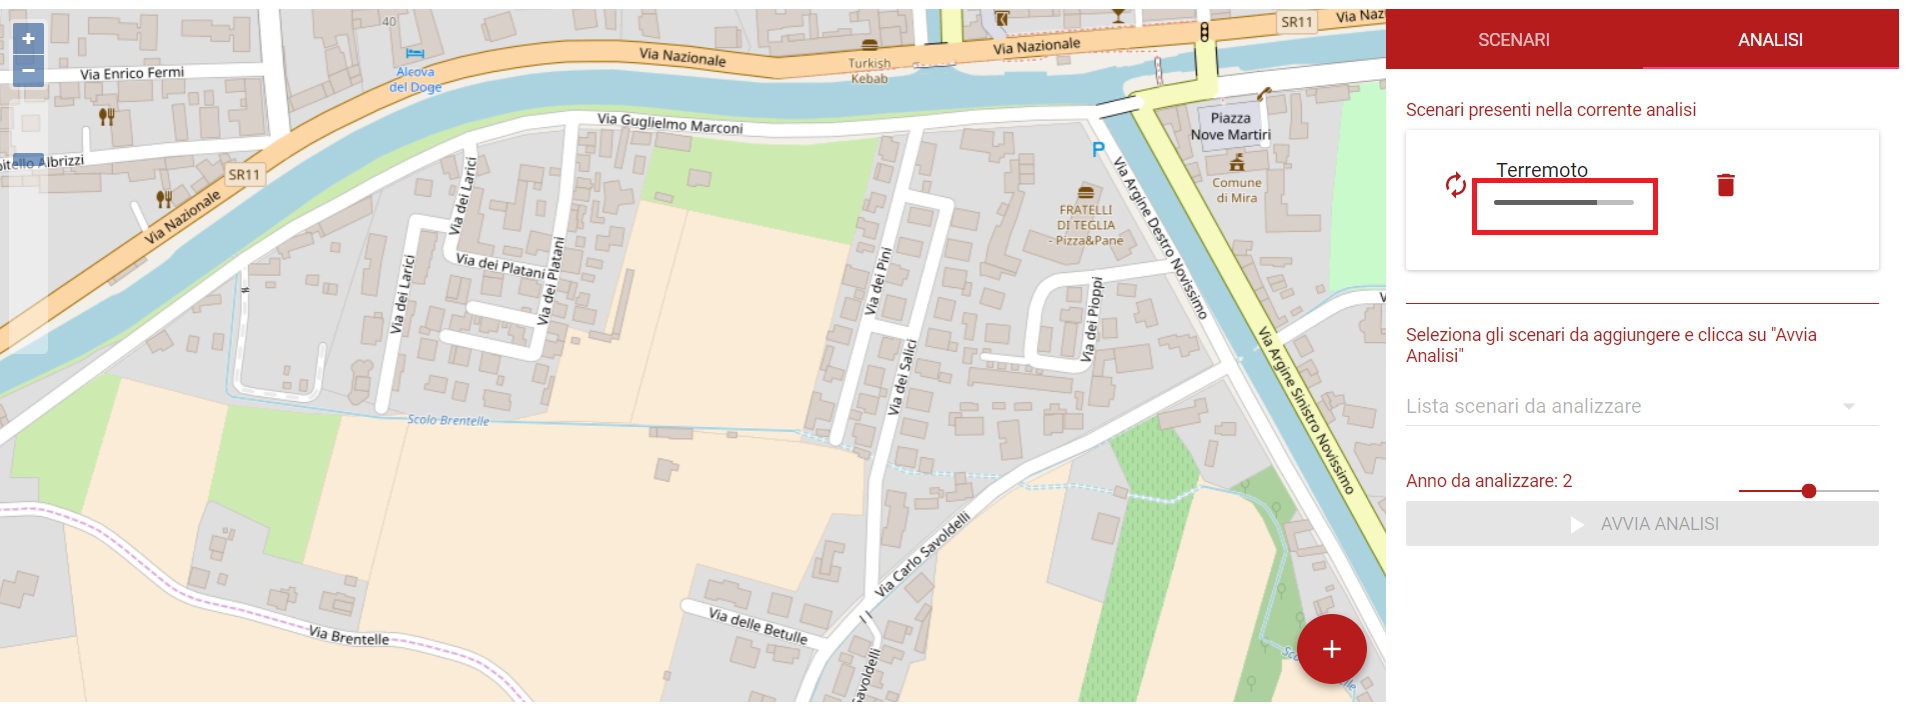
\includegraphics[width=\textwidth]{img/avanzamento_analisi.png}
		\caption{Avanzamento analisi}
	\end{figure}

\subsection{Risultati analisi e legenda}
	Quando l'analisi è completa, viene visualizzata una finestra informativa con i risultati economici dei danni causati dagli scenari presi in esame.
	Inoltre, sulla mappa i nodi assumono vari colori, a seconda della perdita economica che il nodo subisce.\\
	Cliccando sul pulsante "Mostra legenda" è possibile visualizzare una legenda che descrive il significato dei colori.

	\begin{figure}[H]
		\centering
		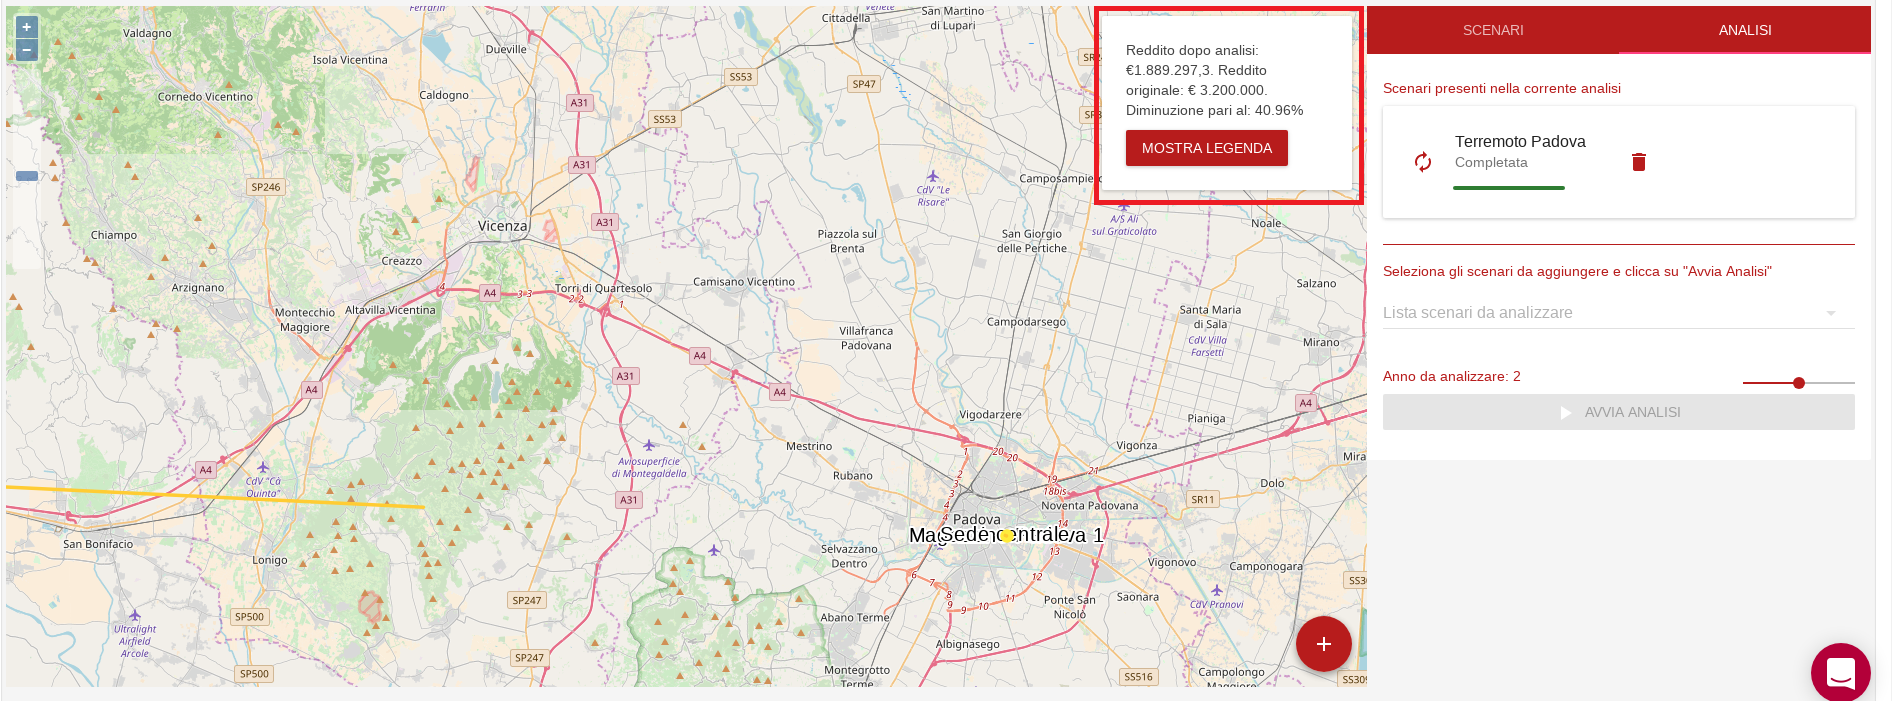
\includegraphics[width=\textwidth]{img/finestra_economica.png}
		\caption{Finestra risultati economici}
	\end{figure}

	\begin{figure}[H]
	\centering
	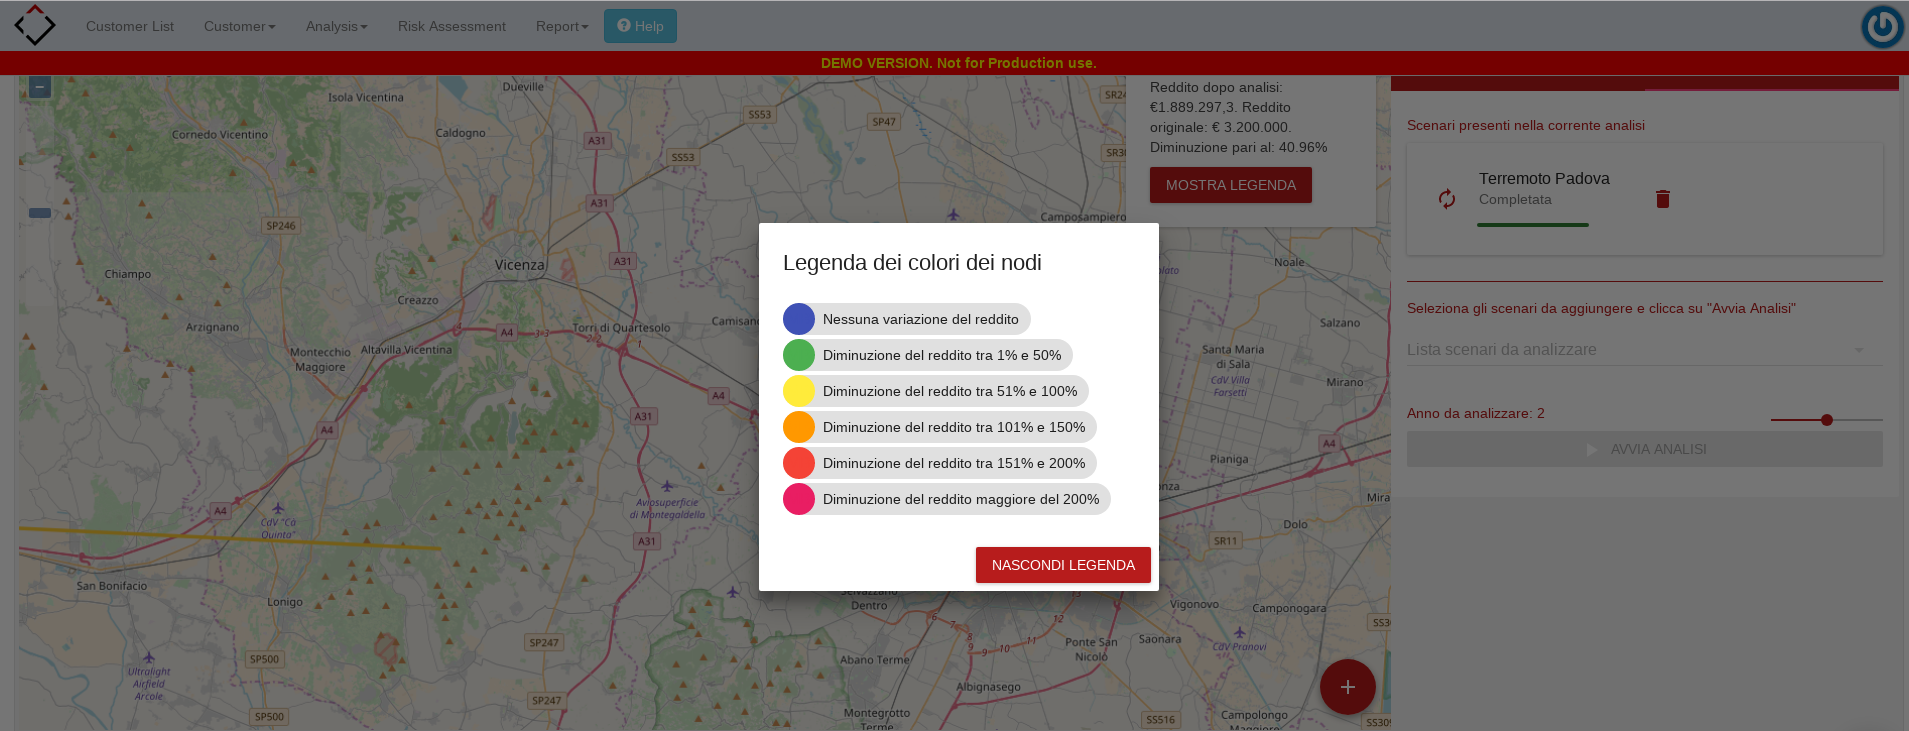
\includegraphics[width=\textwidth]{img/legenda_colori.png}
	\caption{Legenda colori nodi}
	\end{figure}

\subsection{Modifica anno di analisi}
	L'applicazione permette di visualizzare i risultati di danno a uno, due o tre anni a partire dalla data attuale. Per modificare l'anno di analisi, è possibile fare scorrere lo slider presente nella sidebar.
	
	\begin{figure}[H]
		\centering
		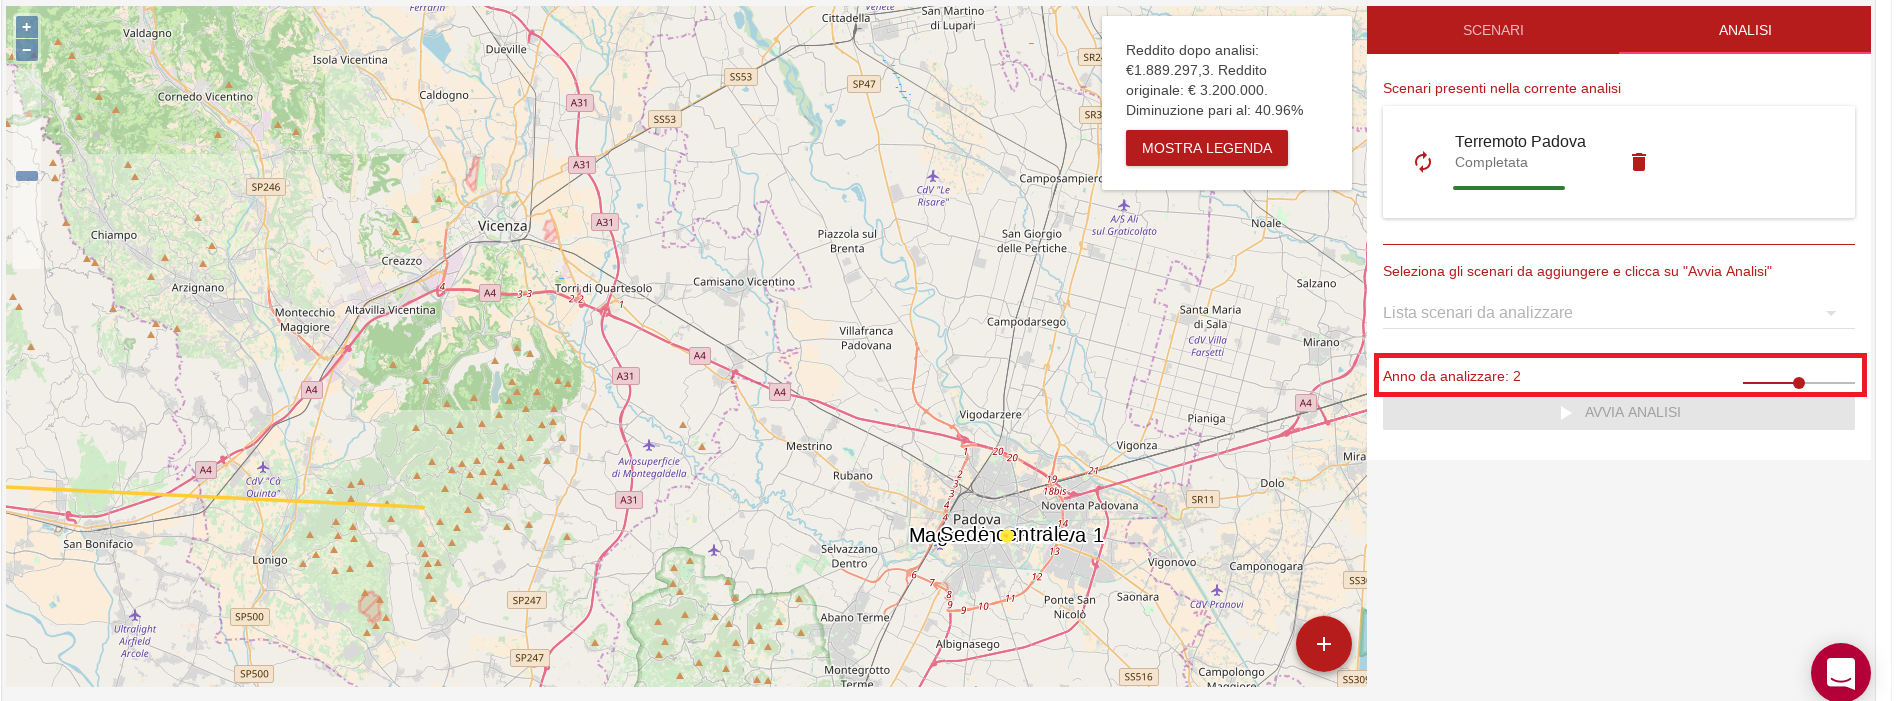
\includegraphics[width=\textwidth]{img/modifica_anno_analisi.png}
		\caption{Modifica anno di analisi}
	\end{figure}

\subsection{Cancellazione risultati di analisi}
	Per cancellare un'analisi, è possibile cliccare sul pulsante a forma di cestino sulla destra di ogni analisi.
	
	\begin{figure}[H]
		\centering
		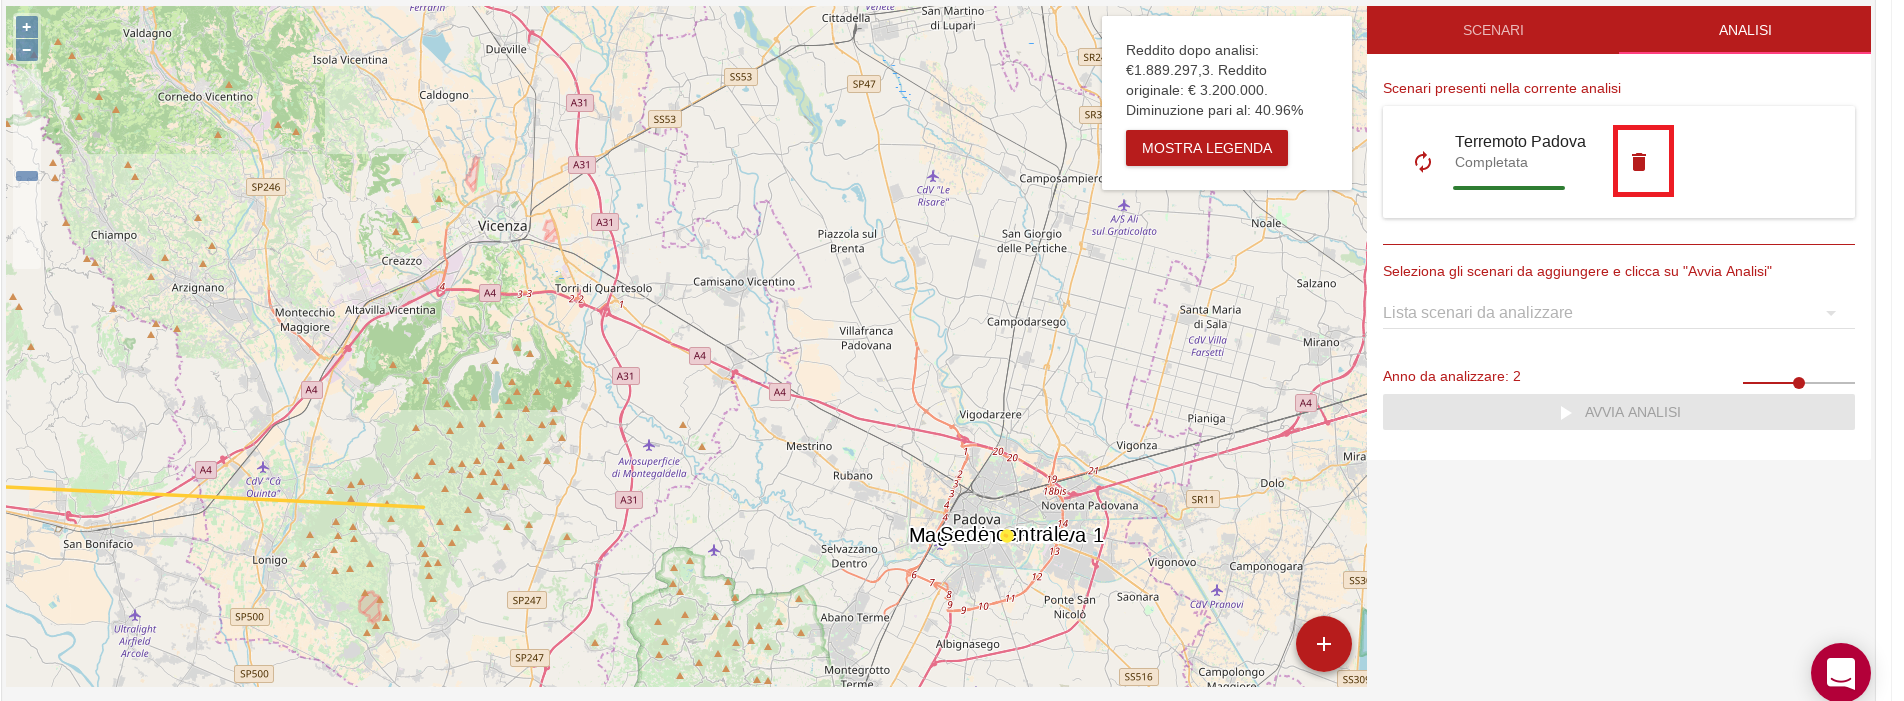
\includegraphics[width=\textwidth]{img/cancellazione_analisi.png}
		\caption{Cancellazione analisi}
	\end{figure}


\subsection{Riesecuzione analisi}
	Qualora i dati del processo produttivo o dello scenario fossero cambiati, è possibile ricalcolare l'analisi premendo sul pulsante con le due frecce a sinistra di ogni analisi.
	
	\begin{figure}[H]
		\centering
		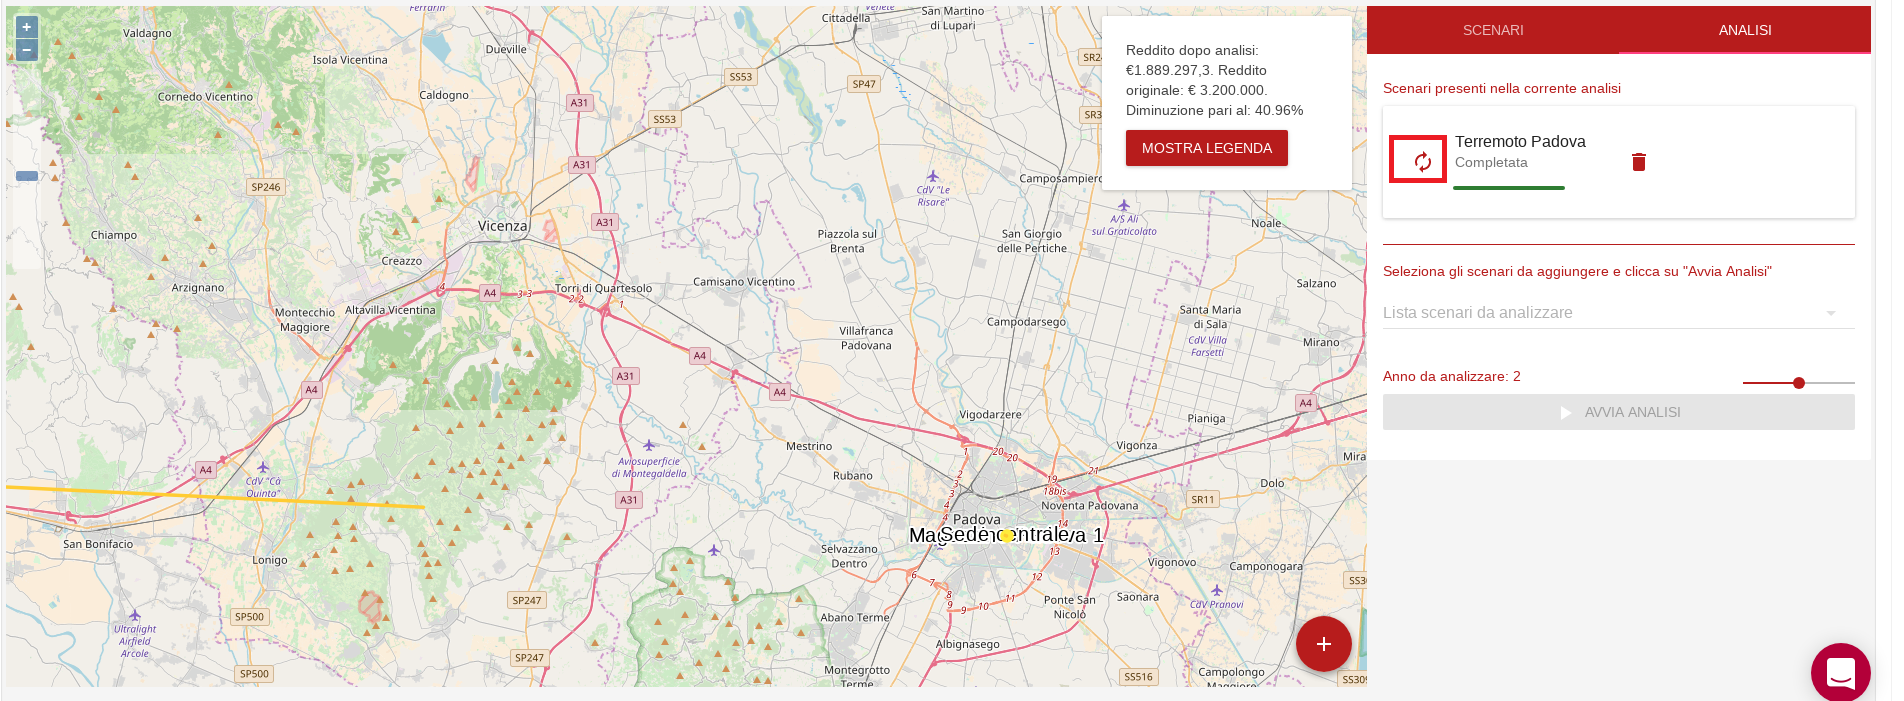
\includegraphics[width=\textwidth]{img/riesecuzione_analisi.png}
		\caption{Riesecuzione analisi}
	\end{figure}


\section{Messaggi d'errore}
	Durante la sua esperienza all'interno di DeGeOP, l'utente può riscontrare errori in fase di compilazione dei dati all'interno della sidebar, in fase di disegno sulla mappa o in caso di errori di connessione.

\subsection{Errori di compilazione dati sulla sidebar}
	In caso di errata compilazione dei dati all'interno della sidebar, viene visualizzato un errore nel box in alto a destra sulla mappa.
	In particolare tutti i campi della sidebar devono essere non vuoti e devono rispettare le regole di validazione descritte nell'apposita appendice \nameref{Validazioni}.
	
\subsection{Errori di disegno sulla mappa}
	In caso di fase di disegno sulla mappa viene visualizzato un errore nel box in alto a destra sulla mappa. Gli errori possono essere:
	\begin{itemize}
		\item il perimetro dell'\mglo{Asset}{asset} non è stato disegnato o non è stato correttamente chiuso facendo coincidere l'ultimo spigolo del perimetro col primo;
		\item il \mglo{Nodo}{nodo} non è stato posizionato all'interno di un asset.
	\end{itemize}
%	TODO
%	\begin{figure}[H]
%	\centering
%	\includegraphics[width=\textwidth]{img/errore_message_wrapper.png}
%	\caption{Visualizzazione messaggio di errore in fase di compilazione dati sulla sidebar o disegno sulla mappa}
%	\end{figure}


\subsection{Errore per mancanza di connessione internet}
	In caso di mancanza di connessione internet l'applicazione continua a funzionare per 5 minuti in modalità \mglo{Offline}{offline}. Se allo scadere di questo tempo continua a non essere presente la connessione, l'utente visualizzerà un messaggio di errore.
	%TODO
%	\begin{figure}[H]
%	\centering
%	\includegraphics[width=\textwidth]{img/errore_no_internet.png}
%	\caption{Visualizzazione del messaggio di connessione assente}
%	\end{figure}

\subsection{Errore per problemi con il server di RiskApp}
	In caso di problemi nel contattare il server di \riskapp{} l'utente visualizzerà istantaneamente un messaggio di errore.
	%TODO
%	\begin{figure}[H]
%	\centering
%	\includegraphics[width=\textwidth]{img/errore_no_server.png}
%	\caption{Visualizzazione del messaggio di errore di connessione col server di RiskApp}
%	\end{figure}
\section{Segnalazione problemi}
%controllare se la mail di zephyrys è questa
Nel caso in cui venissero riscontrati malfunzionamenti del servizio DeGeOP, l'utente ha la possibilità di inviare una mail all'indirizzo:
\begin{center}
	zephyrus-swe@gmail.com
\end{center}
con oggetto \textit{Segnalazione problema DeGeOP}.
Nel corpo della mail devono essere specificati:
	\begin{itemize}
		\item la data in cui si è riscontrato il problema;
		\item una concisa ma completa spiegazione del problema.
	\end{itemize}
Il tuo contributo verrà analizzato quanto prima.
\appendix
\section{Validazioni}
	\label{Validazioni}
	In questa sezione vengono illustrate le condizioni di validità dei campi presenti nella sidebar.
\subsection{Asset}
	%TABELLA: nome_campo | regola_di_validazione
	
	\begin{table}[H]
		\centering
		\begin{tabular}{ p{3cm}p{0cm}p{10.5cm}}
			\toprule
			\textbf{Nome Campo:} & & \textbf{Regola di validazione:} \\
			\midrule
			{Nome} & & Non vuoto; max 50 caratteri; non può iniziare e/o finire con uno spazio; non può contenere caratteri speciali
			\\ \hline
			{Descrizione} & & {Non vuoto; max 5000 caratteri; non può iniziare e/o finire con uno spazio; non può contenere caratteri speciali diversi dall'apostrofo} \\ \hline
			{Tipologia} & &{La scelta della tipologia di costruzione dell'\mglo{Asset}{asset} è obbligatoria} \\ \hline
			{Appartenenza} & &{La scelta dell'appartenenza dell'asset è obbligatoria} \\ \hline
			{Colore} & &{La scelta del colore dell'asset è obbligatoria} \\ \hline
			{Superficie (in mq)} & &{Non vuota; max 5 cifre per la parte intera; max 2 cifre per la parte decimale} \\ \hline
			{Valore unitario (monetario)} & &{Non vuoto; max 20 cifre per la parte intera; max 2 cifre per la parte decimale} \\ \hline
			{Valuta} & &{La scelta della valuta dell'asset è obbligatoria} \\ \hline
		\end{tabular}
		\caption{Condizioni di validità dei campi presenti nella sidebar relativa ad un asset }
	\end{table}

\subsection{Nodo}
	%TABELLA: nome_campo | regola_di_validazione
	
		\begin{table}[H]
			\centering
			\begin{tabular}{ p{3cm}p{0cm}p{10.5cm}}
				\toprule
				\textbf{Nome Campo:} & & \textbf{Regola di validazione:} \\
				\midrule
				{Classe} & & {La scelta della valuta dell'asset è obbligatoria}
				\\ \hline
				{Nome} & & {Non vuoto; max 50 caratteri; non può iniziare e/o finire con uno spazio; non può contenere caratteri speciali} \\ \hline
				{Capacità} & &{Non vuota; max 5 cifre per la parte intera; max 2 cifre per la parte decimale} \\ \hline
				{Tempo di processo} & &{Non vuota; max 4 cifre per l'ora; max 2 cifre per i minuti (comprese tra 0 e 59); max 2 cifre per i secondi (comprese tra 0 e 59)} \\ \hline
				{Valore unitario (monetario)} & &{Non vuoto; max 20 cifre per la parte intera; max 2 cifre per la parte decimale} \\ \hline
				{Tempo di consegna} & &{Non vuota; max 4 cifre per l'ora; max 2 cifre per i minuti (comprese tra 0 e 59); max 2 cifre per i secondi (comprese tra 0 e 59)} \\ \hline
			\end{tabular}
			\caption{Condizioni di validità dei campi presenti nella sidebar relativa ad un \mglo{Nodo}{nodo} }
		\end{table}

%\subsection{Arco
	%visto che l'arco di tipo trasporto non c'è allora non ci sono campi da validare
\section{Glossario}
	\subsection{A}
		\mgref{Arco}
		Collegamento orientato tra due nodi.
		
		\mgref{Asset}
		Fabbricato con importanza strategica per il processo produttivo di un'azienda. Un asset può contenere uno o più nodi.
		
		\mgref{Asus}
		Azienda produttrice di dispositivi tecnologici di varia tipologia.
	\subsection{B}
		\mgref{Browser}
		Il web browser, o più semplicemente browser, è un'applicazione per il recupero, la presentazione e la navigazione di risorse web. Tali risorse (ad esempio pagine web, immagini, video) sono a disposizione sul World Wide Web su una rete locale o sullo stesso computer dove il browser è in esecuzione. 
	\subsection{C}
		\mgref{Chrome}
		\mglo{Browser}{Browser} web sviluppato da Google.
	 %\subsection{D}
%	\subsection{E}
	\subsection{F}
		\mgref{Firefox}
		\mglo{Browser}{Browser} web  libero e multipiattaforma, mantenuto da Mozilla Foundation.
	\subsection{G}
		\mgref{Gesture}
		Combinazione di movimenti e click del dispositivo di puntamento (ad esempio il mouse) che vengono riconosciuti come comandi specifici.
		
		\mgref{Gruppo}
		Componenti che fanno parte del gruppo \zephyrus.
%	\subsection{H}
	\subsection{I}
		\mgref{iOS}
		Sistema operativo sviluppato da Apple Inc.
	
		\mgref{Ipad}
		Tablet prodotto dall'azienda Apple Inc.
%	\subsection{J}
%	\subsection{K}
%	\subsection{L}
		\mgref{Linux}
		Linux è una famiglia di sistemi operativi di tipo Unix-like, rilasciati sotto varie distribuzioni, aventi la caratteristica comune di utilizzare come nucleo il kernel Linux. Ubuntu è la distribuzione di Linux più utilizzata.
	\subsection{M}
		\mgref{MacOS}
		Sistema operativo sviluppato da Apple.
	\subsection{N}
		\mgref{Nodo}
		Oggetto che fa parte dei processo produttivo aziendale. È contenuto all'interno di un asset.
	\subsection{O}
		\mgref{Offline}
		Il dispositivo non è connesso alla rete.
		
%	\subsection{P}
%	\subsection{Q}
%	\subsection{R}
	\subsection{S}
		\mgref{Safari}
		\mglo{Browser}{browser} web sviluppato dalla Apple.
%	\subsection{T}
%	\subsection{U}
%	\subsection{V}
		\mgref{VirtualBox}
		Software open source per l'esecuzione di macchine virtuali.
	\subsection{W}
		\mgref{Windows}
		Sistema operativo sviluppato da Microsoft.
%	\subsection{X}
%	\subsection{Y}
%	\subsection{Z}
%\clearpage

\appendix
\printglossaries

\end{document}


%Manuale utente: come fa l’utente a ottenere copia dell’applicazione?

%LEAF
%Manuale utente: buono, con giusto equilibrio tra immagini e testo. Bene la
%descrizione dettagliata dell’installazione e della procedura di segnalazione dei
%problemi. Completare la descrizione delle funzionalità disponibili.

%
%Manuale utente: Per quale motivo a un utente finale dovrebbero interessare i
%riferimenti informativi tecnologici riportati? §2: indicare la versione minima
%di Android sulla quale il prodotto è assicurato funzionare. Uniformare gli
%screenshot al medesimo look-and-feel. Non chiara la dicitura (Funzionalità
%non presente) su alcune funzionalità: non presente perché non ancora
%sviluppata o perché non verrà supportata? Buono per struttura, ma alcuni degli
%screenshot forniti non sono adeguatamente descritti. Completare.

%AAA Manca completamente un Glossario dedicato.
%AAA Qual è l’URL al quale collegarsi per accedere al sistema? 
%AAA Non è descritto il processo di segnalazione di eventuali errori del prodotto. Il documento è completamente privo di immagini che aiutino l’utente a collegare le descrizioni presenti al prodotto vero e proprio.

%TODO 1) Evidenziare le tecnologie utillzate,
%TODO 2) Strumenti necessari
%TODO 3) Glossario Dedicato
%TODO Estensione funzionalità
%TODO Estensione del codice